% Report Phase 2 - Tox21 toxicity prediction
% Single-file, self-contained report. Build with:  tectonic report_phase2.tex
\documentclass[conference]{IEEEtran}

\usepackage[T1]{fontenc}
\usepackage{mathptmx}   % Times text+math with T1 shapes: IEEEtran's typeface, no substitutions
\usepackage{microtype}
\usepackage{amsmath,amssymb}
\usepackage{graphicx}
\usepackage{booktabs}
\usepackage{multirow}
\usepackage{array}
\usepackage{xcolor}
\usepackage{enumitem}
\usepackage{longtable}
\usepackage[numbers,sort&compress]{natbib}
\usepackage[hidelinks]{hyperref}

\graphicspath{{figures/}{../../results/figures/}}

\setlist{itemsep=2pt,topsep=4pt,parsep=0pt}
\renewcommand{\arraystretch}{1.1}
\setlength{\tabcolsep}{3pt}
\setlength{\emergencystretch}{2em}

\newcommand{\code}[1]{\texttt{\small #1}}

\begin{document}

%--------------------------------------------------------------------
% Title block
%--------------------------------------------------------------------
\title{Molecular Toxicity Prediction with Graph Neural Networks\\ and Hybrid Models}

\author{\IEEEauthorblockN{Hardik Shreyas, Saman, Arjun, Bhavya and Priyansh}
\IEEEauthorblockA{Tox21 Toxicity Prediction Project --- Phase 2}}

\maketitle

\begin{abstract}
We compare classical chemical fingerprints with graph neural networks (GNNs) and hybrid
models for predicting 12 Tox21 toxicity endpoints. All model families share the same cleaned
data, the same seven split files (one deterministic scaffold split, three randomized scaffold
splits and three random splits), and the same endpoint-wise masked ROC-AUC and PR-AUC scorer.
The GNNs are trained with a masked multi-task loss, so an unmeasured assay label contributes
neither loss nor gradient. We evaluate a graph convolutional network (GCN), a bond-aware
message-passing network (MPNN with GINE layers), and AttentiveFP against fingerprint-based
logistic regression, random forest and XGBoost. Three hybrids combine the Morgan fingerprint
with graph information through frozen embeddings, probability stacking, or end-to-end fusion.
On the randomized scaffold splits the best GNN reaches a mean test ROC-AUC of
$0.828$, against $0.839$ for the best fingerprint-plus-descriptor model. The stacking hybrid
reaches $0.836$ and is the only model that an exploratory paired Wilcoxon test cannot separate
from that baseline ($p=0.47$), while beating both of its own parents. End-to-end fusion does
not improve on its parents, and its ablations identify why. A 10\% graph augmentation study
changes neither result. The overall finding is measured: learned molecular graphs are useful,
but they do not replace a well-tuned engineered-feature baseline, and the benefit of combining
representations depends on \emph{how} the combination is trained.
\end{abstract}

\begin{IEEEkeywords}
Tox21, molecular toxicity, molecular fingerprints, graph neural networks, scaffold split,
multi-task learning
\end{IEEEkeywords}

%--------------------------------------------------------------------
\section{Introduction and Objectives}
%--------------------------------------------------------------------
Toxicity prediction from molecular structure is a multi-task learning problem with two
structural difficulties. First, a compound may be tested in some assays but not others, and an
unmeasured endpoint must never be treated as a negative example. Second, the evaluation
protocol decides the answer: a random split can place close analogues of every test molecule in
the training set, whereas a scaffold split holds out whole groups of related molecular
frameworks and therefore measures generalization to new chemistry.

Phase~1 established the classical pipeline on this data: cleaning and deduplication
(7{,}709 unique molecules), deterministic and randomized scaffold splits, Morgan fingerprints
and RDKit descriptors, and logistic regression, random forest and XGBoost tuned on validation
PR-AUC. This phase asks two questions:

\begin{enumerate}[label=\textbf{Q\arabic*.}]
\item Do models that learn directly from the atom--bond graph improve on the engineered-feature
baselines, particularly on unseen scaffolds?
\item Does combining a graph representation with engineered features help, and does the answer
depend on how tightly the two are coupled?
\end{enumerate}

To make the comparison meaningful rather than rhetorical, every model family in this report
shares the same cleaned data, the same seven split files, the same endpoint definitions and the
same masked scorer. Nothing reported here was measured outside that single scorer. Sections
\ref{sec:protocol}--\ref{sec:dl} describe the protocol and the architectures,
Sections~\ref{sec:gnn-results}--\ref{sec:hybrid} report results and ablations, and
Section~\ref{sec:validation} reports the statistical and calibration checks that qualify them.

%--------------------------------------------------------------------
\section{Data and Experimental Protocol}
\label{sec:protocol}
%--------------------------------------------------------------------
\subsection{Dataset}
We use the MoleculeNet/DeepChem release of Tox21: 7{,}831 compounds with 12 binary labels
covering seven nuclear-receptor (NR) and five stress-response (SR) pathways
\citep{wu2018moleculenet}. Each SMILES string is parsed with RDKit, reduced to its largest
fragment to strip salts and counter-ions, and canonicalized; charges and stereochemistry are
retained. Duplicates are merged on canonical SMILES \emph{before} splitting, and labels that
disagree within a duplicate group are set to missing (44 such molecule--endpoint pairs, a direct
measure of assay noise). The result is 7{,}709 unique molecules with 2{,}285 Bemis--Murcko
scaffolds \citep{bemis1996murcko}.

Two properties of the label matrix shape every design decision that follows. Positive rates run
from 2.9\% (NR-PPAR-gamma) to 15.9\% (SR-ARE), so accuracy is uninformative and PR-AUC must be
read against each endpoint's prevalence. And 17\% of the matrix is missing --- between 7\% and
26\% per endpoint --- because a compound was not tested, not because it was inactive.
Missingness is not random: larger molecules are labelled on fewer endpoints
(Spearman $\rho=-0.39$).

\begin{figure}[t]
\centering
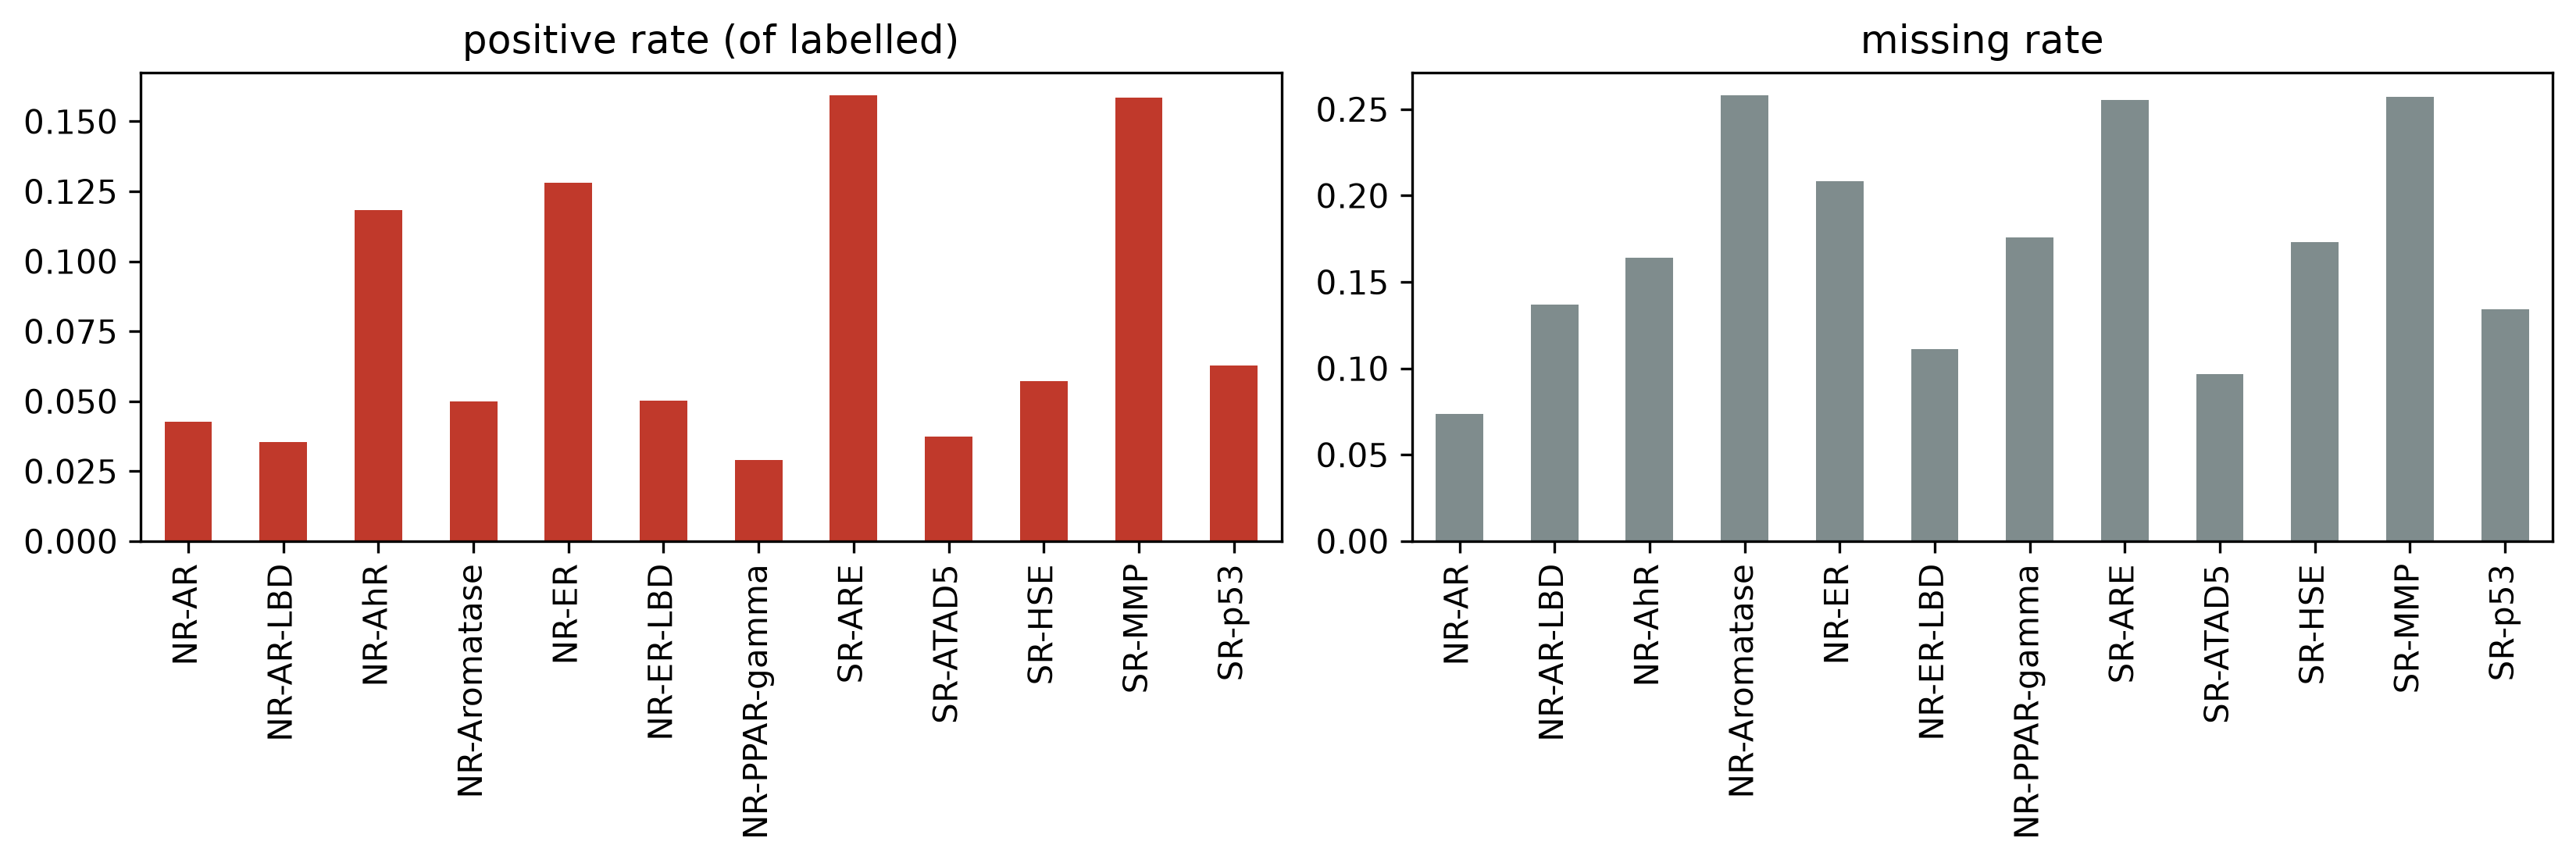
\includegraphics[width=0.78\textwidth]{eda_label_rates.png}
\caption{Positive rate (among labelled molecules) and missing rate for each of the 12 endpoints.
Both the imbalance and the missingness vary substantially across endpoints.}
\label{fig:labels}
\end{figure}

\subsection{Splits}
Seven split files are shared by every model in this report:

\begin{itemize}
\item \code{scaffold\_det} --- one deterministic Bemis--Murcko scaffold split
(6{,}167 train / 770 validation / 772 test molecules), used for hyper-parameter tuning and for
all ablations, so that ablation arms differ only in the ablated factor.
\item \code{scaffold\_s0}--\code{scaffold\_s2} --- three randomized scaffold splits, reported as
the ``scaffold'' column; this family is the headline generalization test.
\item \code{random\_s0}--\code{random\_s2} --- three random splits, reported as ``random'';
the gap to the scaffold family is the \emph{generalization penalty}.
\end{itemize}

\subsection{Metrics and the masking rule}
A single scorer (\code{tox.metrics}) is used for every model, classical or deep. For each
endpoint it drops the molecules whose label is missing and computes ROC-AUC and PR-AUC on the
remainder; endpoints that cannot be scored in a given split (no positives or no negatives) are
excluded from that run's mean. Because PR-AUC depends on prevalence, it is comparable only
within a column: the random-classifier level is $0.103$ on the scaffold splits and $0.077$ on
the random splits.

Model selection is on validation only. Hyper-parameters, early stopping and the choice of
reported configuration all use validation data; test labels are read exactly once per run, after
training has finished.

%--------------------------------------------------------------------
\section{Background and Related Work}
%--------------------------------------------------------------------
\textbf{Graph convolutional networks.} \citet{kipf2017gcn} derive a convolution for
graph-structured data from a first-order approximation of spectral graph convolutions; its cost
grows linearly with the number of edges. Here it is the simplest message-passing baseline: it
averages neighbours with a degree normalization and has no input for bond types.

\textbf{Expressive power.} \citet{xu2019gin} characterize the discriminative power of
message-passing networks, showing that popular variants such as GCN and GraphSAGE fail to
distinguish some simple structures, and propose the Graph Isomorphism Network, whose power
matches the Weisfeiler--Lehman isomorphism test. This motivates \emph{summing} rather than
averaging neighbour messages in our bond-aware model.

\textbf{Edge-aware layers.} \citet{hu2020pretrain} study pre-training GNNs at node and
whole-graph level and report gains of up to 9.4\% absolute ROC-AUC on molecular property and
protein-function prediction, with limited or negative transfer when only one level is
pre-trained. The edge-feature variant of the GIN layer introduced there is implemented as
\code{GINEConv} in PyTorch Geometric \citep{fey2019pyg} and is what we use to feed bond features
into the messages. We do not use pre-training.

\textbf{Depth and over-smoothing.} \citet{li2018oversmooth} show that GCN propagation is a form
of Laplacian smoothing, which explains both why it works and why stacking many layers can make
vertex features indistinguishable. \citet{oono2020expressive} analyse GCNs as dynamical systems
and prove that, under conditions on the weights, a deep network's output retains only connected
components and node degrees. These are asymptotic results on citation-style graphs; whether
depth hurts molecular graphs of median diameter nine bonds at 2--5 layers is an empirical
question, which our layer ablation tests directly.

\textbf{Position in the molecular literature.} Message passing was unified for chemistry by
\citet{gilmer2017mpnn}, and AttentiveFP \citep{xiong2020attentivefp} adds attention at the atom
and molecule level. \citet{yang2019analyzing} caution that well-tuned fingerprint baselines are
often competitive with learned representations --- which is why this report measures the graph
models against the classical ones on identical splits instead of assuming they win.

%--------------------------------------------------------------------
\section{Architecture Logic}
\label{sec:arch}
%--------------------------------------------------------------------
\subsection{Molecules as graphs}
A molecule is an undirected graph $G=(V,E)$ whose nodes are heavy atoms and whose edges are
bonds. Each atom $v$ carries a feature vector $x_v\in\{0,1\}^{36}$ and each bond $\{u,v\}$ a
vector $e_{uv}\in\{0,1\}^{6}$. The atom features are one-hot blocks for atomic number (12 listed
elements plus ``other''), degree 0--5, formal charge $\{-1,0,+1,\text{other}\}$, hybridization
$\{$SP, SP$^2$, SP$^3$, SP$^3$D, SP$^3$D$^2$, other$\}$ and total hydrogen count 0--4, plus
aromatic and in-ring flags. The bond features are bond type (single, double, triple, aromatic)
with conjugated and in-ring flags. Every undirected bond is stored as two directed edges with
identical features, which is what lets a message flow both ways. The labels of one molecule form
a vector $y\in\{0,1,\mathrm{NaN}\}^{12}$; missing labels stay NaN and are masked in the loss
rather than filled. Chirality and bond stereochemistry are not encoded.

\subsection{Message passing and readout}
Following the message-passing framework of \citet{gilmer2017mpnn}, a layer updates every atom
from its bonded neighbours $\mathcal N(v)$:
\begin{equation}
h_v^{(l+1)}=\phi\Big(h_v^{(l)},\ \mathop{\mathrm{AGG}}_{u\in\mathcal N(v)}\ \psi\big(h_u^{(l)},e_{uv}\big)\Big),
\qquad h_v^{(0)}=x_v .
\end{equation}
After $L$ layers, atom $v$ depends on every atom within $L$ bonds of it, so $L$ sets the size of
the chemical neighbourhood the model can see. A \emph{readout} then maps the variable-size set
of atom vectors to one fixed-size molecule vector. For GCN and MPNN we concatenate the mean and
the element-wise maximum over atoms,
\begin{equation}
g=\Big[\tfrac1{|V|}\textstyle\sum_{v}h_v^{(L)}\ \Big\|\ \max_{v}h_v^{(L)}\Big],
\end{equation}
because the mean summarizes overall composition independently of molecule size, while the
maximum records whether \emph{any} atom strongly expresses a feature --- the natural form of a
toxicophore, a local substructure that is either present or not. A shared head
($\to 128 \to 12$, ReLU, dropout) turns $g$ into 12 logits.

\subsection{The three architectures and why they are compared}
The three architectures are chosen to isolate one design axis each: fixed aggregation without
bonds, bond-aware summation, and learned attention.

\textbf{GCN} \citep{kipf2017gcn}. One layer is
$H'=\sigma(\hat D^{-1/2}\hat A\hat D^{-1/2}HW)$ with $\hat A=A+I$: each atom takes a
degree-normalized average of itself and its neighbours, followed by one shared linear map. It is
the simplest message-passing model and it \emph{ignores bond features}, so it is the baseline
against which any benefit of bond information or attention is measured.

\textbf{MPNN with GINE layers.} Our \code{mpnn} uses the edge-aware GIN layer introduced for
molecules by \citet{hu2020pretrain},
\begin{equation}
h_v'=\mathrm{MLP}\Big((1+\epsilon)\,h_v+\sum_{u\in\mathcal N(v)}\mathrm{ReLU}\big(h_u+W e_{uv}\big)\Big),
\end{equation}
where $\epsilon$ is learned and $W$ projects the 6-dimensional bond vector to the atom-feature
width. Two properties motivate it. Bonds enter the message through $We_{uv}$, so a double bond
and an aromatic bond send different messages, which GCN cannot express. And it \emph{sums} over
neighbours before an MLP, which \citet{xu2019gin} show is as discriminative as the
1-dimensional Weisfeiler--Lehman test, whereas mean or degree-normalized aggregation can map
different neighbourhoods to the same vector (one neighbour versus two identical neighbours). It
uses the same BatchNorm--ReLU--dropout block, readout and head as GCN.

\textbf{AttentiveFP} \citep{xiong2020attentivefp}. Neighbour messages are weighted by learned
attention coefficients, atom states are updated with GRU cells, and the molecule vector is built
by repeatedly attending over all atoms (2 readout time steps). It replaces the fixed mean$\|$max
readout with a learned one, and is included as the strongest published graph baseline for
molecular property prediction.

\subsection{Over-smoothing: a hypothesis, not an assumption}
Stacking message-passing layers makes the atom representations of a connected graph more alike.
For GCN this is exact in the linear case: $\hat D^{-1/2}\hat A\hat D^{-1/2}$ is a low-pass
filter \citep{li2018oversmooth}, and \citet{oono2020expressive} prove that a deep GCN's output
converges to a subspace determined only by connected components and node degrees. But those are
statements about depth tending to infinity in citation-type graphs. Molecules are small: in the
cleaned Tox21 set the median molecule has 16 heavy atoms and a graph diameter of 9 bonds (95th
percentile 19), and only 19\% of molecules have diameter $\le 5$. At 2--5 layers we are far from
the asymptotic regime, and even a 5-layer model does not see the whole molecule from every atom
for most compounds. We therefore state over-smoothing as a hypothesis and test it with the layer
ablation in Section~\ref{sec:gnn-results}.

\subsection{Masked multi-task loss}
Let $m_{ij}\in\{0,1\}$ indicate that label $y_{ij}$ of molecule $i$ and endpoint $j$ is observed,
let $z_{ij}$ be the logit and $p_{ij}=\sigma(z_{ij})$. Treating the observed labels as
independent Bernoulli variables and weighting the positive term by $w_j$, the negative
log-likelihood of the observed entries is
\begin{equation}
\mathcal L = -\frac{1}{\sum_{i,j}m_{ij}}\sum_{i,j}m_{ij}\Big[
w_j\,y_{ij}\log p_{ij}+(1-y_{ij})\log(1-p_{ij})\Big].
\end{equation}
Differentiating with respect to the logit gives
\begin{equation}
\frac{\partial\mathcal L}{\partial z_{ij}}
=\frac{m_{ij}}{\sum m}\Big[(1-y_{ij})\,p_{ij}-w_j\,y_{ij}\,(1-p_{ij})\Big],
\end{equation}
which is exactly zero whenever $m_{ij}=0$: a missing label contributes neither loss nor
gradient. Filling missing entries with 0 would instead assert that \emph{unmeasured} means
\emph{non-toxic} and push every endpoint towards the negative class. In the implementation NaN
labels are replaced by a dummy 0 \emph{before} the cross-entropy, so no NaN is ever evaluated,
and the result is multiplied by the mask; a batch with no labels at all returns 0 through the
clamp $\max(\sum m,1)$.

The positive weight is $w_j=\min(n^-_j/n^+_j,30)$, computed on training labels only, which
counteracts the 3--16\% positive rates; the cap keeps the gradient of very rare endpoints
bounded. Dividing by the total number of observed entries rather than per endpoint means
endpoints with more labels contribute more to the gradient.

\emph{Why multi-task.} Related endpoints share structure --- our exploratory analysis finds
strong correlation between NR-AR/NR-AR-LBD and NR-ER/NR-ER-LBD --- and sharing a representation
can help the sparse endpoints \citep{caruana1997multitask,mayr2016deeptox}. This is a hypothesis
for our data, tested by the multi-task versus 12 single-task ablation.
\emph{Caveat.} Ignoring missing labels is unbiased for the observed-label objective only if
missingness is unrelated to the label given the molecule; assay selection in Tox21 is not random,
so some bias is possible.

%--------------------------------------------------------------------
\section{Deep Learning Models and Training Protocol}
\label{sec:dl}
%--------------------------------------------------------------------
The three models (\code{gcn}, \code{mpnn}, \code{afp}) are implemented in PyTorch with PyTorch
Geometric \citep{fey2019pyg} on the cleaned data and the same seven split files as the classical
models. Every model outputs 12 logits per molecule; probabilities are $\sigma(\text{logit})$ and
are written in the shared prediction format, so the common scorer scores them exactly as it
scores the fingerprint models.

\textbf{Optimization.} Adam \citep{kingma2015adam} with learning rate $10^{-3}$, weight decay
$10^{-5}$, batch size 64, at most 200 epochs, minimizing the masked weighted binary
cross-entropy of Section~\ref{sec:arch}. Random seeds for Python, NumPy and PyTorch are set
together, and the shuffling of the training set depends only on (seed, epoch), so an interrupted
run resumes to an identical result. Every epoch is checkpointed (weights, optimizer, random
generators, early-stopping counters), and a run is skipped when its prediction file already
exists.

\textbf{Early stopping and model selection.} After each epoch the mean validation ROC-AUC over
the scorable endpoints is computed with the shared scorer. Training stops when it has not
improved for 25 epochs, and the weights of the best epoch are restored. Validation PR-AUC is
logged at the same epoch and is the only criterion used to choose between hyper-parameter
settings. The test set is predicted once, after the best weights are restored; no choice ---
stopping, epoch, hyper-parameters or ablation arm --- uses test labels.

\textbf{Hyper-parameter tuning.} For each architecture all 12 combinations of hidden width
$\{64,128,256\}$, depth $\{3,4\}$ and dropout $\{0.1,0.3\}$ were trained on \code{scaffold\_det}
with seed 0 and validation data only, and the combination with the highest validation PR-AUC was
frozen (Table~\ref{tab:hparams}). The frozen setting is then used unchanged on every split and
seed. Tuning with a single seed is a budget decision: differences between neighbouring
configurations smaller than the seed-to-seed spread reported below should not be
over-interpreted.

\begin{table}[t]
\centering
\caption{Frozen configurations, selected on \code{scaffold\_det} validation PR-AUC (seed 0,
36 trials in total). The selected setting is then used unchanged on all seven splits.}
\label{tab:hparams}
\small
\begin{tabular}{lcccc}
\toprule
model & hidden width & layers & dropout & val.\ PR-AUC at selection \\
\midrule
gcn  & 256 & 3 & 0.1 & 0.429 \\
mpnn & 256 & 4 & 0.1 & 0.384 \\
afp  & 256 & 3 & 0.3 & 0.414 \\
\bottomrule
\end{tabular}
\end{table}

\textbf{Final runs.} Each architecture is trained nine times: \code{scaffold\_det} with seeds
0, 1, 2, and each balanced scaffold split \code{scaffold\_s}$k$ and random split
\code{random\_s}$k$ with seed $k$ --- the same convention as the classical grid, so that every
reported number is a mean over three runs.

\begin{figure}[t]
\centering
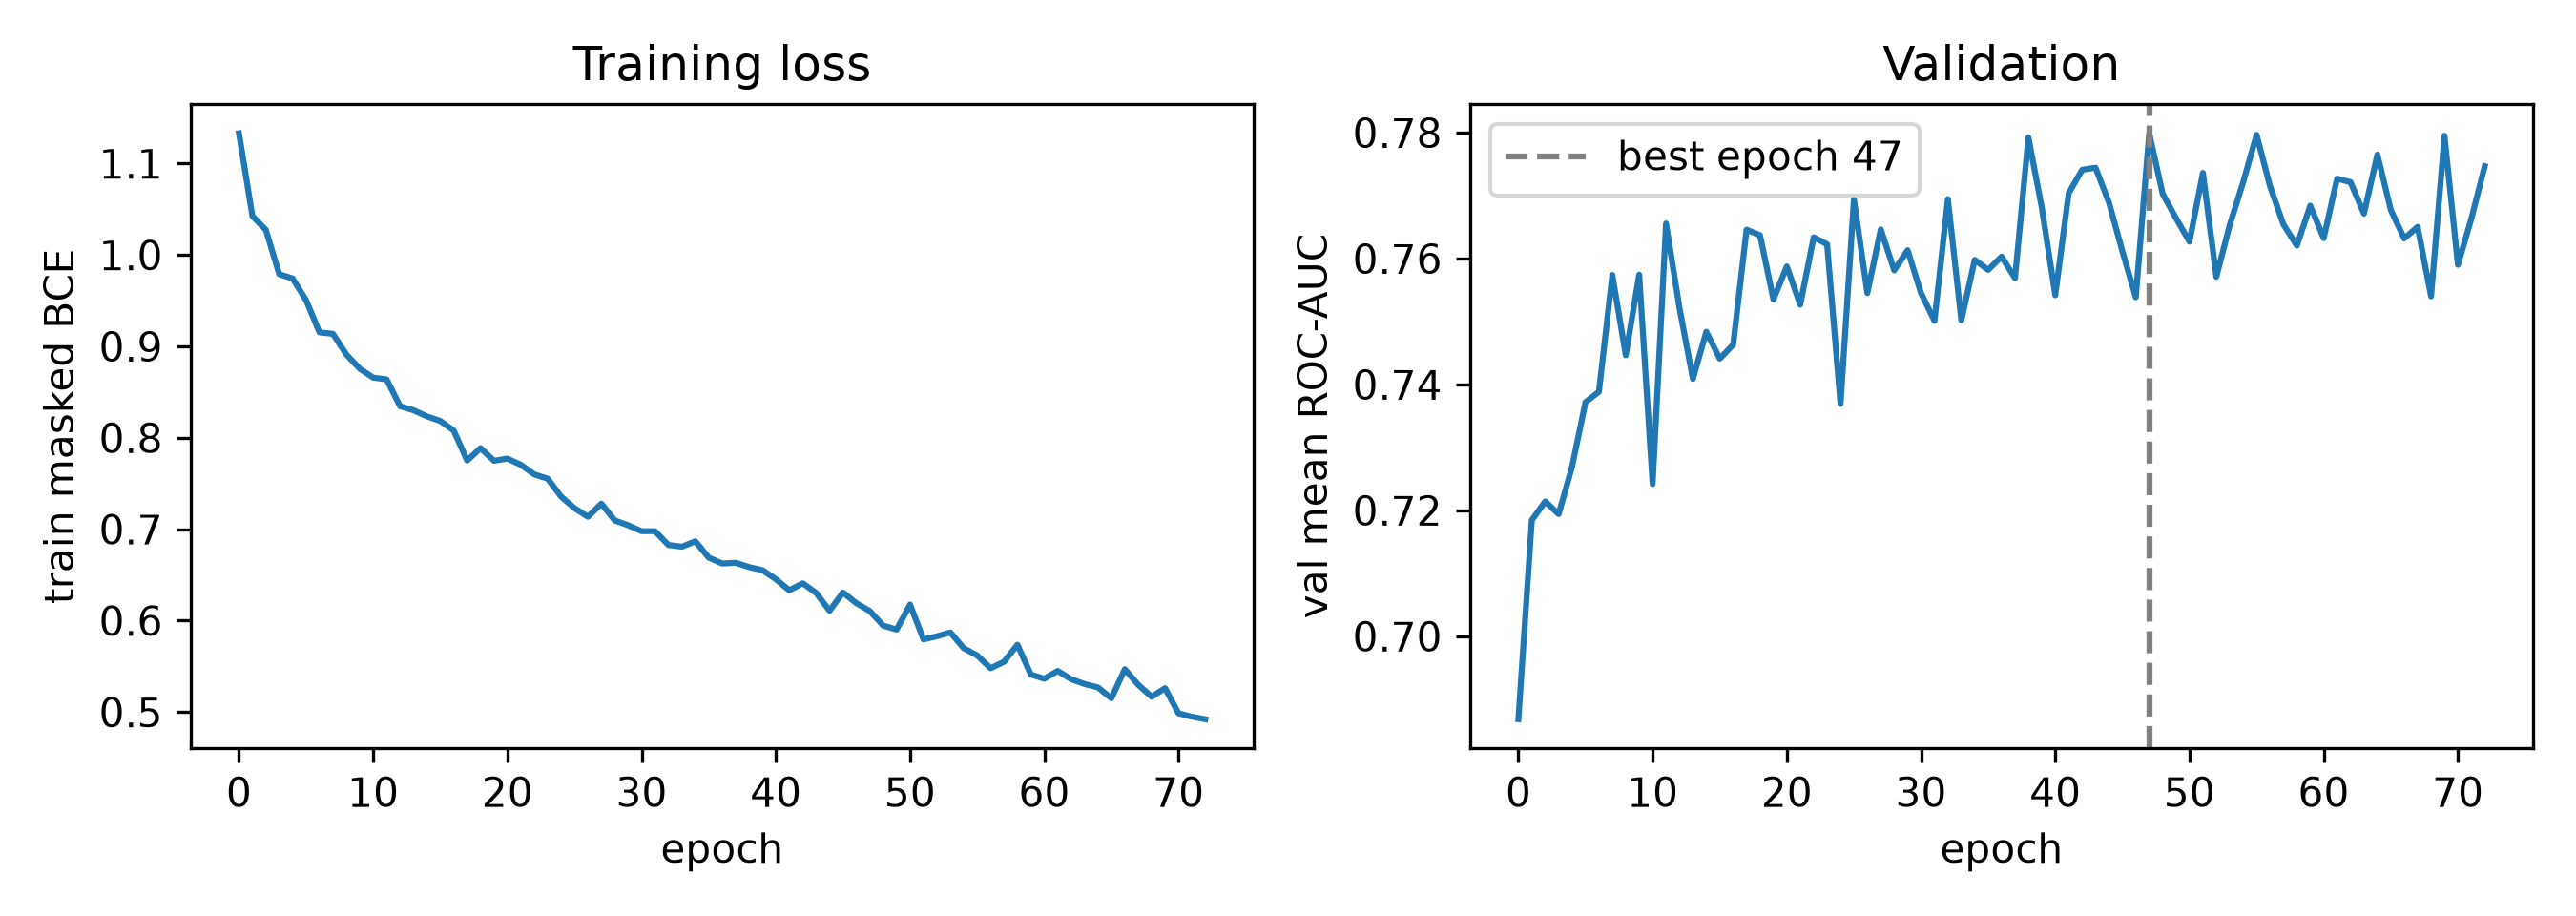
\includegraphics[width=\textwidth]{mpnn__scaffold_det__seed0_curve.png}
\caption{A representative training run (\code{mpnn}, \code{scaffold\_det}, seed 0). The masked
training loss falls steadily while validation ROC-AUC plateaus and becomes noisy; the dashed line
marks the epoch whose weights are restored. Training continues for 25 further epochs before
stopping, which is why the curve extends past the selected epoch.}
\label{fig:curve}
\end{figure}

%--------------------------------------------------------------------
\section{Results: Graph Networks}
\label{sec:gnn-results}
%--------------------------------------------------------------------
\subsection{Main comparison}
Table~\ref{tab:gnn-main} reports the three graph models beside the six classical models on all
three split families.

\begin{table*}[t]
\centering
\caption{Test ROC-AUC and PR-AUC, 12-endpoint mean, mean $\pm$ std over 3 runs
(\code{scaffold\_det}: seeds 0--2; \code{scaffold} and \code{random}: the three seeded splits).
PR-AUC is comparable only within a column; the bottom row gives the random-classifier level.}
\label{tab:gnn-main}
\footnotesize
\setlength{\tabcolsep}{3.5pt}
\resizebox{\textwidth}{!}{%
\begin{tabular}{lcccccc}
\toprule
 & \multicolumn{3}{c}{ROC-AUC} & \multicolumn{3}{c}{PR-AUC} \\
\cmidrule(lr){2-4}\cmidrule(lr){5-7}
model & scaffold\_det & scaffold & random & scaffold\_det & scaffold & random \\
\midrule
gcn & 0.752 $\pm$ 0.007 & 0.826 $\pm$ 0.016 & 0.842 $\pm$ 0.008 & 0.354 $\pm$ 0.004 & 0.446 $\pm$ 0.052 & 0.460 $\pm$ 0.023 \\
mpnn & 0.732 $\pm$ 0.011 & 0.813 $\pm$ 0.020 & 0.831 $\pm$ 0.007 & 0.309 $\pm$ 0.014 & 0.386 $\pm$ 0.014 & 0.435 $\pm$ 0.049 \\
afp & 0.769 $\pm$ 0.002 & 0.828 $\pm$ 0.017 & 0.844 $\pm$ 0.010 & 0.354 $\pm$ 0.011 & 0.419 $\pm$ 0.052 & 0.457 $\pm$ 0.009 \\
\midrule
lr\_fp & 0.715 $\pm$ 0.000 & 0.775 $\pm$ 0.036 & 0.801 $\pm$ 0.013 & 0.319 $\pm$ 0.000 & 0.395 $\pm$ 0.051 & 0.435 $\pm$ 0.038 \\
lr\_fpdesc & 0.722 $\pm$ 0.000 & 0.788 $\pm$ 0.039 & 0.826 $\pm$ 0.010 & 0.299 $\pm$ 0.000 & 0.367 $\pm$ 0.068 & 0.463 $\pm$ 0.029 \\
rf\_fp & 0.732 $\pm$ 0.001 & 0.803 $\pm$ 0.019 & 0.833 $\pm$ 0.009 & 0.366 $\pm$ 0.001 & 0.442 $\pm$ 0.043 & 0.484 $\pm$ 0.019 \\
rf\_fpdesc & \textbf{0.782 $\pm$ 0.003} & \textbf{0.839 $\pm$ 0.024} & 0.862 $\pm$ 0.002 & \textbf{0.406 $\pm$ 0.002} & \textbf{0.481 $\pm$ 0.043} & \textbf{0.531 $\pm$ 0.016} \\
xgb\_fp & 0.696 $\pm$ 0.003 & 0.767 $\pm$ 0.045 & 0.801 $\pm$ 0.012 & 0.306 $\pm$ 0.006 & 0.389 $\pm$ 0.047 & 0.435 $\pm$ 0.024 \\
xgb\_fpdesc & 0.761 $\pm$ 0.008 & 0.813 $\pm$ 0.032 & 0.855 $\pm$ 0.007 & 0.391 $\pm$ 0.008 & 0.446 $\pm$ 0.057 & 0.520 $\pm$ 0.020 \\
\midrule
\multicolumn{4}{l}{positive rate (random-classifier PR-AUC)} & 0.103 & 0.103 & 0.077 \\
\bottomrule
\end{tabular}}
\end{table*}

Three observations follow. First, all three graph models beat the fingerprint-only classical
models (\code{lr\_fp}, \code{rf\_fp}, \code{xgb\_fp}) on every split family, so learning the
representation from the graph does recover real signal. Second, none of them beats
\code{rf\_fpdesc}, the fingerprint-plus-descriptor random forest, which remains the strongest
single model on all three families. Third, the ordering among the graph models is not the
ordering their design would suggest: AttentiveFP leads, plain GCN is close behind, and the
bond-aware MPNN is last --- which is what makes the ablations below worth reading.

Every model loses roughly 0.02--0.03 ROC-AUC moving from random to randomized scaffold splits,
and considerably more on the harder deterministic scaffold split, confirming that the split
protocol, not the architecture, dominates apparent performance.

\subsection{Ablations}
All five ablations use \code{mpnn} --- the architecture whose defining feature, bond
information, is one of the ablated factors --- on \code{scaffold\_det} with seeds 0--2, changing
one factor at a time relative to the frozen model: (i) 2, 3, 4 or 5 message-passing layers;
(ii) bond features zeroed (\code{mpnn-noedge}); (iii) mean, max or mean$\|$max readout;
(iv) twelve independent single-endpoint models instead of one multi-task model; and (v) the
positive-class weights switched off. Because the frozen \code{mpnn} has 4 layers
(Table~\ref{tab:hparams}), the \code{mpnn-l4} arm reproduces the baseline exactly, which is a
useful internal consistency check. In the single-endpoint arm each of the 12 models has its own
initialization, early stopping on its own endpoint, and its own weight.

\begin{table}[t]
\centering
\caption{MPNN ablations on \code{scaffold\_det}: test ROC-AUC and PR-AUC (12-endpoint mean,
mean $\pm$ std over 3 seeds). One factor changes per arm; the baseline is the frozen
\code{mpnn}.}
\label{tab:gnn-ablation}
\small
\begin{tabular}{llcc}
\toprule
group & arm & ROC-AUC & PR-AUC \\
\midrule
baseline & mpnn (4 layers) & 0.732 $\pm$ 0.011 & 0.309 $\pm$ 0.014 \\
\midrule
layers & mpnn-l2 & \textbf{0.747 $\pm$ 0.003} & 0.328 $\pm$ 0.004 \\
layers & mpnn-l3 & 0.741 $\pm$ 0.003 & 0.319 $\pm$ 0.006 \\
layers & mpnn-l4 & 0.732 $\pm$ 0.011 & 0.309 $\pm$ 0.014 \\
layers & mpnn-l5 & 0.731 $\pm$ 0.011 & 0.313 $\pm$ 0.017 \\
\midrule
bond features & mpnn-noedge & 0.743 $\pm$ 0.011 & 0.320 $\pm$ 0.006 \\
readout & mpnn-pmax & 0.743 $\pm$ 0.006 & 0.321 $\pm$ 0.017 \\
readout & mpnn-pmean & 0.743 $\pm$ 0.016 & 0.324 $\pm$ 0.003 \\
positive weights & mpnn-nopw & 0.746 $\pm$ 0.007 & \textbf{0.345 $\pm$ 0.023} \\
multi-task & mpnn-single & 0.747 $\pm$ 0.000 & 0.320 $\pm$ 0.010 \\
\bottomrule
\end{tabular}
\end{table}

The ablations (Table~\ref{tab:gnn-ablation}) read uncomfortably but honestly: \emph{every arm
scores at or above the frozen baseline}.

\begin{itemize}
\item \textbf{Depth.} Test ROC-AUC decreases monotonically from 2 to 5 layers
(0.747, 0.741, 0.732, 0.731). The direction is consistent with the over-smoothing hypothesis of
Section~\ref{sec:arch}, but the effect is small, it is also consistent with plain overfitting of
a larger model on 6{,}167 training molecules, and 2--5 layers is far from the asymptotic regime
those theorems describe. We therefore record the direction and decline to claim the mechanism.
\item \textbf{Bond features.} Zeroing the bond features \emph{improves} the model
(0.743 vs 0.732). The feature that distinguishes this architecture from GCN does not pay for
itself here --- consistent with the main table, where bond-aware MPNN trails bond-blind GCN.
\item \textbf{Readout.} Mean alone and max alone both slightly beat the concatenation, so the
richer readout is not earning its extra width on this data.
\item \textbf{Positive weights.} Switching off the class weighting improves both ROC-AUC and
PR-AUC (0.345 vs 0.309 PR-AUC). The weighting was intended to help the rare endpoints; measured,
it hurts.
\item \textbf{Multi-task.} Twelve single-endpoint models match or beat the shared model
(0.747 vs 0.732). The shared-representation hypothesis is not supported for \code{mpnn} on this
data, though the single-task arm uses twelve times the training compute.
\end{itemize}

The honest reading is that the frozen \code{mpnn} configuration --- selected on a single seed by
validation PR-AUC --- is not the best MPNN available, and that the tuning budget, not the graph
formalism, is the binding constraint. Because every arm is \code{mpnn}-based, these conclusions
are stated for \code{mpnn} only; GCN or AttentiveFP could answer differently.

%--------------------------------------------------------------------
\section{DL Dataset and Regularization}
\label{sec:regularization}
%--------------------------------------------------------------------
Four mechanisms regularize the graph models, all fixed before any test label is read: dropout
$0.2$ after every message-passing block and inside the head; weight decay $10^{-5}$ in Adam;
early stopping on validation mean ROC-AUC with patience 25, which caps the effective number of
epochs (the frozen models stop between epoch 30 and 61 of a 200-epoch budget); and the masked
multi-task loss itself, which makes the twelve endpoints share one encoder so that no single
sparse endpoint can drive the representation on its own. Batch normalisation between layers is
used for optimisation stability rather than for regularization.

\subsection{Augmentation study}
We asked whether graph augmentation adds anything on top of these. Two augmentations are applied
to \emph{training batches only}, so validation and test molecules, early stopping and every
reported metric still describe unperturbed structures:

\begin{itemize}
  \item \code{gcn-augmask} --- \textbf{random atom masking}, 10\%: the feature vector of a
        randomly chosen 10\% of atoms is zeroed. The atom and its bonds stay in the graph, so
        topology, the batch vector and the pooling denominators are unchanged; only the atom's
        identity is hidden, and the model must infer it from its neighbourhood.
  \item \code{gcn-augdrop} --- \textbf{random bond dropping}, 10\%: 10\% of bonds are deleted
        with their features. Both directions of a bond are removed together, so the graph stays
        undirected as the message passing assumes.
\end{itemize}

Both are re-sampled every epoch from the checkpointed random state, so a resumed run replays the
same augmentations. Everything else --- architecture, frozen hyper-parameters, loss, optimiser,
early stopping, seeds --- is identical to the baseline, which is the un-augmented \code{gcn} run
of Table~\ref{tab:gnn-main}. The three arms therefore differ in exactly one factor.

\begin{table}[t]
\centering
\caption{Graph augmentation on \code{scaffold\_det}: test ROC-AUC and PR-AUC, 12-endpoint mean,
mean $\pm$ std over seeds 0--2. The mean test positive rate is $0.103$, which is the PR-AUC of a
random classifier.}
\label{tab:augmentation}
\begin{tabular}{lcc}
\toprule
Arm & ROC-AUC & PR-AUC \\
\midrule
\code{gcn} (no augmentation) & $0.752 \pm 0.008$ & $0.354 \pm 0.004$ \\
\code{gcn-augmask} (atom masking 10\%) & $0.749 \pm 0.005$ & $0.358 \pm 0.005$ \\
\code{gcn-augdrop} (bond dropping 10\%) & $0.753 \pm 0.005$ & $0.340 \pm 0.022$ \\
\bottomrule
\end{tabular}
\end{table}

\textbf{Neither augmentation helps.} Every difference in Table~\ref{tab:augmentation} is smaller
than the seed-to-seed spread beside it. Atom masking costs $0.003$ ROC-AUC and gains $0.004$
PR-AUC; bond dropping gains $0.001$ ROC-AUC and loses $0.014$ PR-AUC with a PR-AUC standard
deviation ($0.022$) five times the baseline's, i.e.\ it mostly adds variance. With three seeds and
differences this small we claim no ordering between the three arms: 10\% augmentation neither
helps nor hurts this model on this split.

That is coherent with the rest of the evidence rather than disappointing. Augmentation treats
over-fitting, and over-fitting is not what limits this model. The GCN already stops early, and in
the ablation grid of Table~\ref{tab:gnn-ablation} every arm but one --- including the
deliberately weakened ones, such as bond features removed or positive weights switched off ---
scores at or above the frozen baseline (the exception is the five-layer arm, $0.731$ against
$0.732$, a gap far inside its own spread). A model that does not degrade when it is weakened is
limited by its tuning budget, not by excess capacity, so there is no over-fitting for
augmentation to remove.

%--------------------------------------------------------------------
\section{Hybrid Models}
\label{sec:hybrid}
%--------------------------------------------------------------------
\subsection{Rationale and the three variants}
The two parents make different mistakes. Fingerprint models encode a fixed vocabulary of
substructures, so they are strong on scaffolds they have seen variations of and weak on
genuinely new chemistry; graph networks learn task-specific representations from the same
training rows, but with 3--16\% positives per endpoint they overfit the sparse endpoints. If the
error profiles differ enough, combining them should help most on the sparse endpoints and on the
low-similarity test molecules. That is a testable claim, and
Section~\ref{sec:hybrid-ablation} tests it. We combine the parents three ways, in increasing
order of coupling:

\begin{description}[style=unboxed,leftmargin=0pt,font=\normalfont\bfseries]
\item[\code{hyb\_embxgb} --- frozen embeddings.] The pooled readout vector of the frozen, tuned
MPNN (encoder weights from the same split and seed, so trained on this split's training rows
only) is concatenated with the 2048-bit Morgan fingerprint, and one XGBoost model is fitted per
endpoint on the concatenation, tuned on validation PR-AUC exactly like the Phase~1 grid.
\item[\code{hyb\_stack} --- probability stacking.] A per-endpoint logistic regression is fitted
on the \emph{validation} probabilities of \code{xgb\_fpdesc} and \code{mpnn} and applied to test.
The meta-learner is never fitted on test. Endpoints whose validation labels do not contain both
classes have nothing to learn; for them the stack falls back to the mean of the two parents.
\item[\code{hyb\_fusion} --- end-to-end fusion.] The Morgan fingerprint goes through a small MLP
branch, the graph through the MPNN encoder branch (warm-started from the checkpoint of the same
split and seed), the two vectors are concatenated before one shared head, and the whole network
is trained end to end with the masked weighted BCE, the Adam recipe of Section~\ref{sec:dl} and
the same early stopping.
\end{description}

Two rules keep the comparison honest: the GNN encoder is only ever used with weights trained on
the same split's training part --- reusing an encoder trained on all data would leak --- and the
stacking meta-learner is fitted on validation, never on test. Every hybrid is reported against
both parents on the same splits and seeds.

\subsection{Final comparison}
Table~\ref{tab:hybrid-main} and Figure~\ref{fig:comparison} give the final comparison on the
shared splits and scorer.

\begin{figure*}[t]
\centering
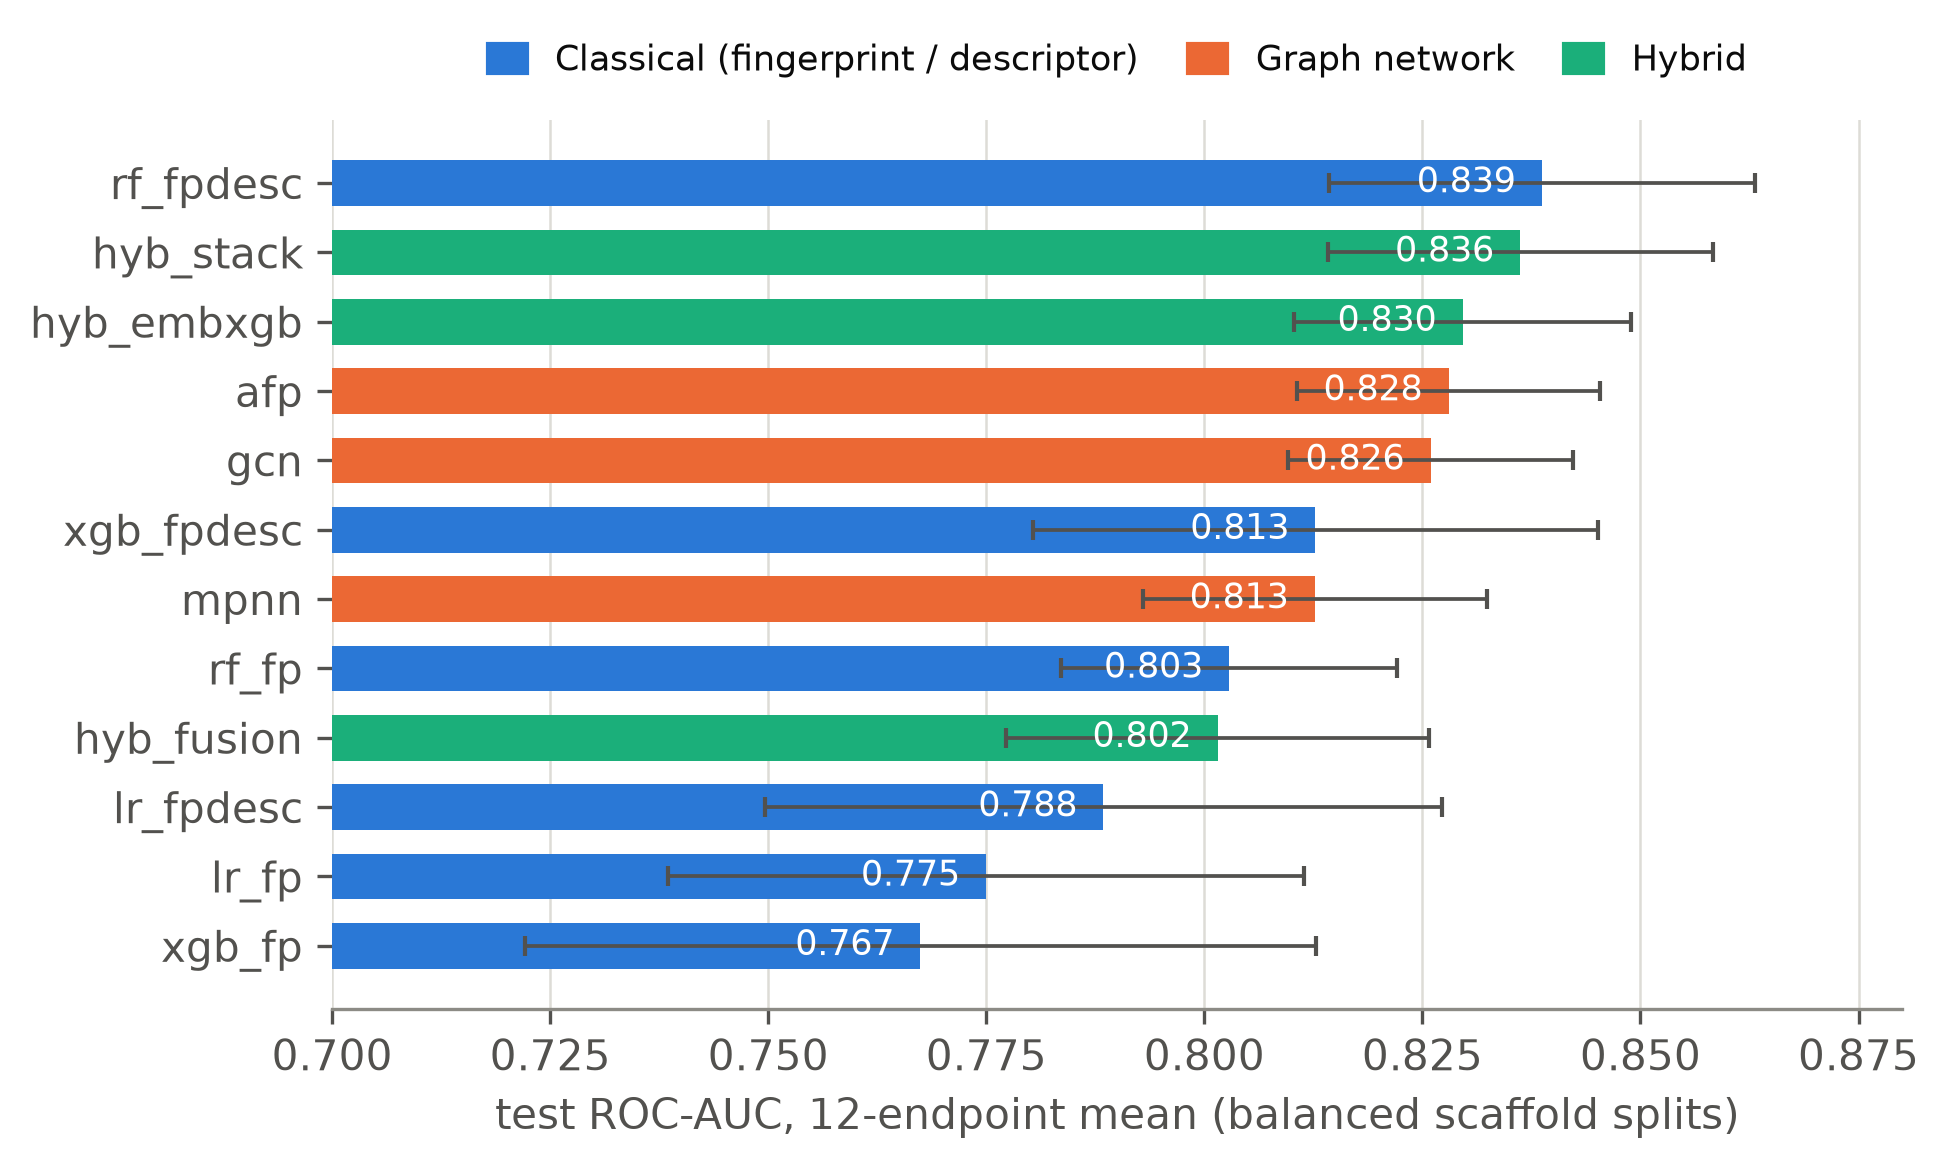
\includegraphics[width=\textwidth]{phase2_model_comparison.png}
\caption{Test ROC-AUC (12-endpoint mean $\pm$ std over the three runs) on the balanced scaffold
splits, the headline generalization test. The best classical model leads, the stacking hybrid is
within one standard deviation of it, and end-to-end fusion falls back into the middle of the
field.}
\label{fig:comparison}
\end{figure*}

\begin{table*}[t]
\centering
\caption{Final Phase~2 comparison: test ROC-AUC and PR-AUC, 12-endpoint mean, mean $\pm$ std
over 3 runs. All models share the splits, the fingerprints and the scorer; the hybrids differ
only in how the two parents are combined.}
\label{tab:hybrid-main}
\footnotesize
\setlength{\tabcolsep}{3.5pt}
\resizebox{\textwidth}{!}{%
\begin{tabular}{lcccccc}
\toprule
 & \multicolumn{3}{c}{ROC-AUC} & \multicolumn{3}{c}{PR-AUC} \\
\cmidrule(lr){2-4}\cmidrule(lr){5-7}
model & scaffold\_det & scaffold & random & scaffold\_det & scaffold & random \\
\midrule
lr\_fp & 0.715 $\pm$ 0.000 & 0.775 $\pm$ 0.036 & 0.801 $\pm$ 0.013 & 0.319 $\pm$ 0.000 & 0.395 $\pm$ 0.051 & 0.435 $\pm$ 0.038 \\
lr\_fpdesc & 0.722 $\pm$ 0.000 & 0.788 $\pm$ 0.039 & 0.826 $\pm$ 0.010 & 0.299 $\pm$ 0.000 & 0.367 $\pm$ 0.068 & 0.463 $\pm$ 0.029 \\
rf\_fp & 0.732 $\pm$ 0.001 & 0.803 $\pm$ 0.019 & 0.833 $\pm$ 0.009 & 0.366 $\pm$ 0.001 & 0.442 $\pm$ 0.043 & 0.484 $\pm$ 0.019 \\
rf\_fpdesc & \textbf{0.782 $\pm$ 0.003} & \textbf{0.839 $\pm$ 0.024} & 0.862 $\pm$ 0.002 & \textbf{0.406 $\pm$ 0.002} & \textbf{0.481 $\pm$ 0.043} & \textbf{0.531 $\pm$ 0.016} \\
xgb\_fp & 0.696 $\pm$ 0.003 & 0.767 $\pm$ 0.045 & 0.801 $\pm$ 0.012 & 0.306 $\pm$ 0.006 & 0.389 $\pm$ 0.047 & 0.435 $\pm$ 0.024 \\
xgb\_fpdesc & 0.761 $\pm$ 0.008 & 0.813 $\pm$ 0.032 & 0.855 $\pm$ 0.007 & 0.391 $\pm$ 0.008 & 0.446 $\pm$ 0.057 & 0.520 $\pm$ 0.020 \\
\midrule
gcn & 0.752 $\pm$ 0.007 & 0.826 $\pm$ 0.016 & 0.842 $\pm$ 0.008 & 0.354 $\pm$ 0.004 & 0.446 $\pm$ 0.052 & 0.460 $\pm$ 0.023 \\
mpnn & 0.732 $\pm$ 0.011 & 0.813 $\pm$ 0.020 & 0.831 $\pm$ 0.007 & 0.309 $\pm$ 0.014 & 0.386 $\pm$ 0.014 & 0.435 $\pm$ 0.049 \\
afp & 0.769 $\pm$ 0.002 & 0.828 $\pm$ 0.017 & 0.844 $\pm$ 0.010 & 0.354 $\pm$ 0.011 & 0.419 $\pm$ 0.052 & 0.457 $\pm$ 0.009 \\
\midrule
hyb\_fusion & 0.748 $\pm$ 0.008 & 0.802 $\pm$ 0.024 & 0.833 $\pm$ 0.008 & 0.311 $\pm$ 0.020 & 0.376 $\pm$ 0.035 & 0.475 $\pm$ 0.036 \\
hyb\_embxgb & 0.742 $\pm$ 0.009 & 0.830 $\pm$ 0.019 & 0.843 $\pm$ 0.008 & 0.336 $\pm$ 0.006 & 0.441 $\pm$ 0.048 & 0.495 $\pm$ 0.035 \\
hyb\_stack & 0.768 $\pm$ 0.006 & 0.836 $\pm$ 0.022 & \textbf{0.864 $\pm$ 0.002} & 0.396 $\pm$ 0.006 & 0.465 $\pm$ 0.038 & 0.529 $\pm$ 0.022 \\
\midrule
\multicolumn{4}{l}{positive rate (random-classifier PR-AUC)} & 0.103 & 0.103 & 0.077 \\
\bottomrule
\end{tabular}}
\end{table*}

Three findings survive the seed spread and the Wilcoxon tests of
Section~\ref{sec:validation}.

\begin{enumerate}
\item \textbf{The graph models close most, but not all, of the gap.} On the randomized scaffold
splits they reach 0.813--0.828 mean test ROC-AUC against the classical models' 0.775--0.839, and
all three beat the fingerprint-only models; but \code{rf\_fpdesc} stays ahead of every graph
model (Wilcoxon $p=0.02$--$0.03$), in line with what \citet{yang2019analyzing} report for
well-tuned fingerprint baselines.
\item \textbf{Stacking is the hybrid that works.} \code{hyb\_stack} beats both of its parents on
the scaffold and random families (parents 0.813 and 0.813 on the scaffold splits; the stack
0.836) and is the only model the Wilcoxon test cannot separate from \code{rf\_fpdesc}
($p=0.47$). On the random splits it is numerically ahead (0.864 vs 0.862), within the seed
spread.
\item \textbf{End-to-end fusion is a negative result with a clear cause.} \code{hyb\_fusion}
reaches 0.748/0.311 (ROC/PR) on \code{scaffold\_det}, below both parents. Fine-tuning the whole
256-unit encoder at the GNN recipe's learning rate $10^{-3}$ degrades within a few epochs, so
early stopping freezes the epoch-0 or epoch-1 warm-start weights in 7 of 9 runs. The ablations
locate the failure: removing the fingerprint branch changes almost nothing (0.744), while
removing the graph branch collapses the model to 0.671 --- the joint head alone cannot learn
what the fingerprints know.
\end{enumerate}

\subsection{Ablations and where the gains come from}
\label{sec:hybrid-ablation}
Five ablations ask what each part contributes; all run on \code{scaffold\_det} with seeds 0--2
and change one factor at a time relative to the main run of the same variant
(Table~\ref{tab:hybrid-ablation}): fusion without the fingerprint branch, fusion without the
graph branch, a fine-tuned rather than frozen encoder in \code{hyb\_embxgb}, performance on the
4 sparsest versus the 4 densest endpoints, and performance by Tanimoto-similarity bin.

\begin{table}[t]
\centering
\caption{Hybrid ablations on \code{scaffold\_det}: test ROC-AUC and PR-AUC (12-endpoint mean,
mean $\pm$ std over 3 seeds). One factor changes per arm; the baseline is the main run of the
same variant.}
\label{tab:hybrid-ablation}
\small
\begin{tabular}{llcc}
\toprule
variant & arm & ROC-AUC & PR-AUC \\
\midrule
hyb\_stack & baseline & 0.768 $\pm$ 0.006 & 0.396 $\pm$ 0.006 \\
\midrule
hyb\_embxgb & baseline (frozen encoder) & 0.742 $\pm$ 0.009 & 0.336 $\pm$ 0.006 \\
hyb\_embxgb & fine-tuned encoder & 0.749 $\pm$ 0.005 & 0.352 $\pm$ 0.014 \\
\midrule
hyb\_fusion & baseline & 0.748 $\pm$ 0.008 & 0.311 $\pm$ 0.020 \\
hyb\_fusion & no fingerprint branch & 0.744 $\pm$ 0.009 & 0.322 $\pm$ 0.010 \\
hyb\_fusion & no graph branch & 0.671 $\pm$ 0.005 & 0.266 $\pm$ 0.006 \\
\bottomrule
\end{tabular}
\end{table}

\begin{table}[t]
\centering
\caption{Test ROC-AUC on the 4 sparsest versus the 4 densest endpoints (\code{scaffold\_det},
mean $\pm$ std over seeds), the direct test of the hybrid rationale: combining two parents should
help most where labels are rare. Selected models; the full table is in
Appendix~\ref{app:sparse}.}
\label{tab:sparse-short}
\small
\begin{tabular}{lcc}
\toprule
model & 4 sparsest endpoints & 4 densest endpoints \\
\midrule
rf\_fpdesc & \textbf{0.786 $\pm$ 0.046} & 0.791 $\pm$ 0.073 \\
afp & 0.764 $\pm$ 0.040 & 0.778 $\pm$ 0.085 \\
mpnn & 0.728 $\pm$ 0.040 & 0.745 $\pm$ 0.070 \\
hyb\_stack & 0.755 $\pm$ 0.022 & \textbf{0.789 $\pm$ 0.081} \\
hyb\_embxgb & 0.742 $\pm$ 0.043 & 0.757 $\pm$ 0.073 \\
hyb\_fusion & 0.760 $\pm$ 0.034 & 0.751 $\pm$ 0.063 \\
\bottomrule
\end{tabular}
\end{table}

\begin{figure}[t]
\centering
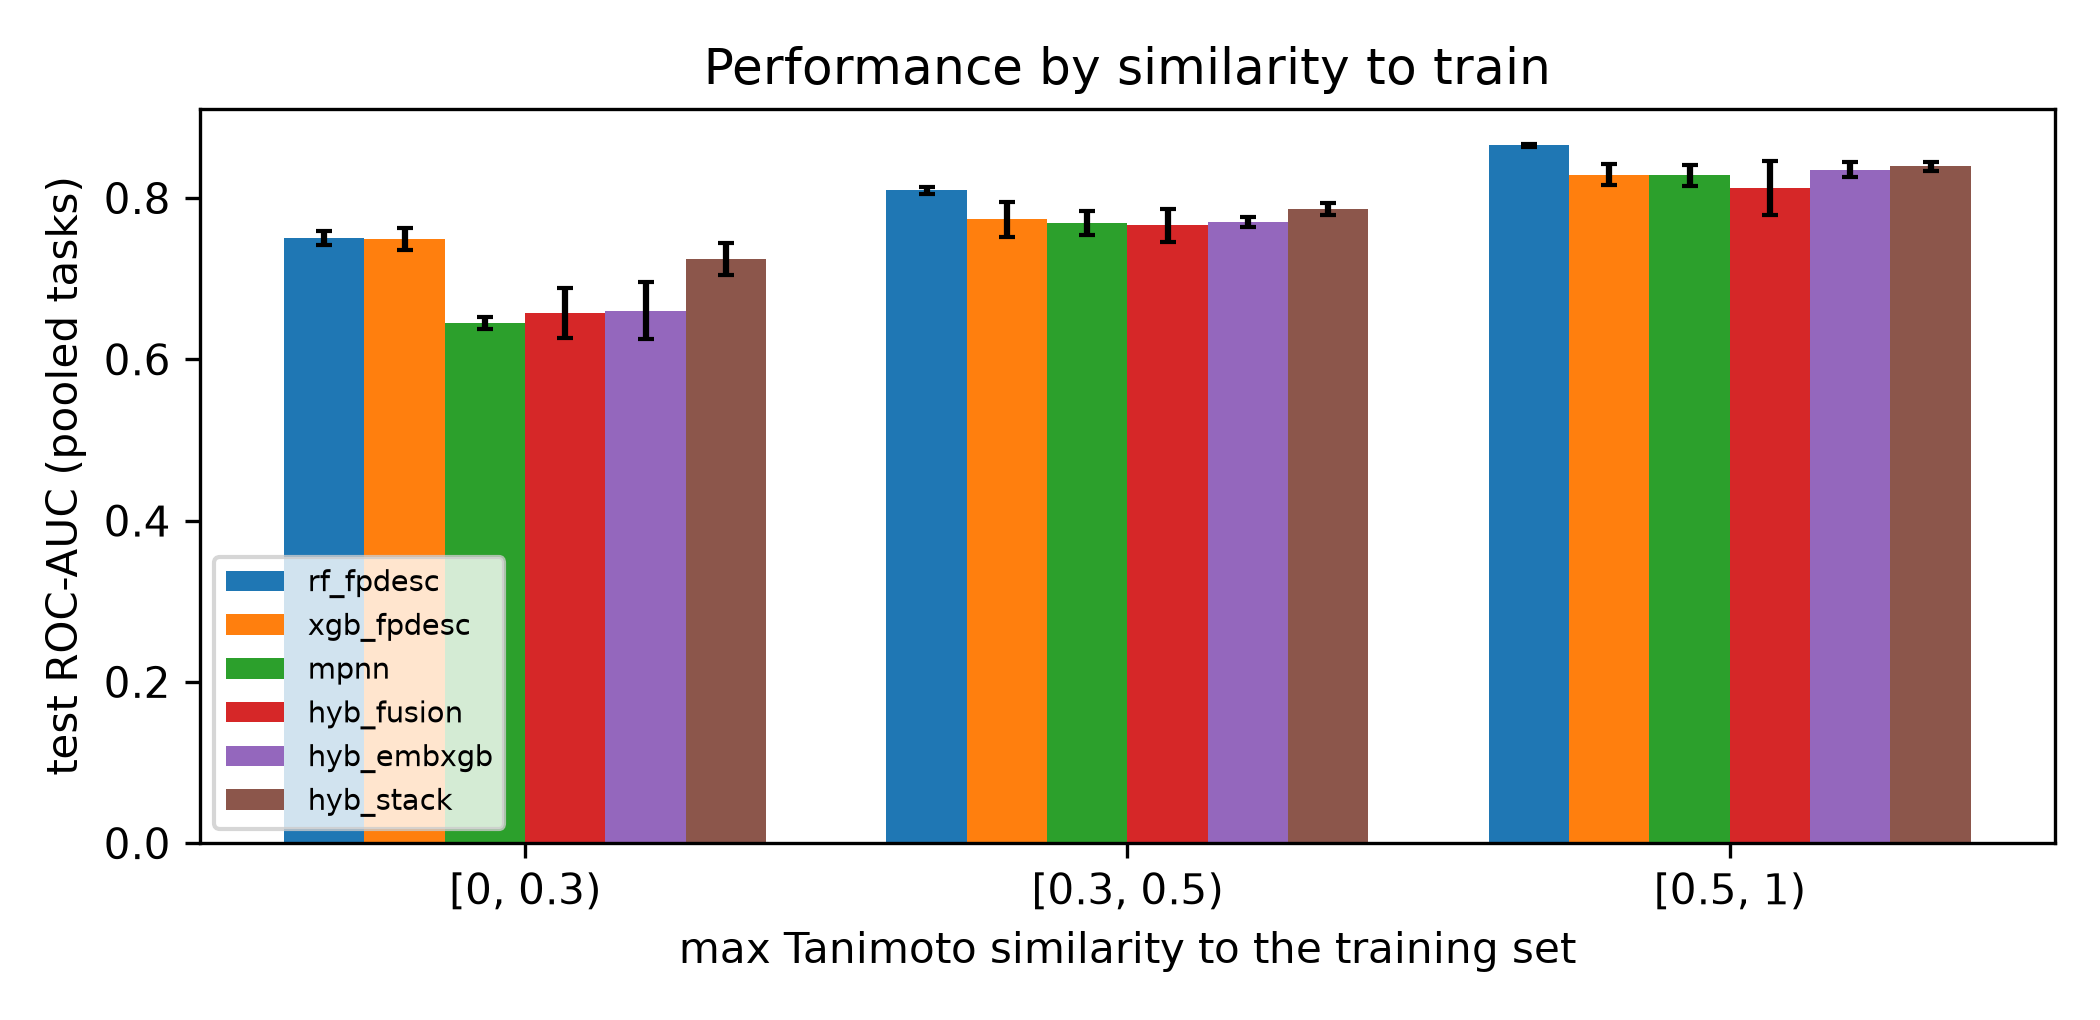
\includegraphics[width=0.92\textwidth]{hybrid_sim_bins.png}
\caption{Test ROC-AUC (all 12 tasks pooled) by the maximum Tanimoto similarity of each test
molecule to the training set (\code{scaffold\_det}). The leftmost bin holds the 172 genuinely
novel molecules. \code{hyb\_stack} clearly beats its graph parent there (0.724 vs 0.645), but
\code{rf\_fpdesc} is stronger still (0.751).}
\label{fig:simbins}
\end{figure}

The similarity analysis (Figure~\ref{fig:simbins}, full numbers in Appendix~\ref{app:simbins})
is where the stated rationale meets the data. Every model degrades sharply on the
$[0,0.3)$ bin, as it should. Within that bin \code{hyb\_stack} (0.724) clearly beats its graph
parent \code{mpnn} (0.645) --- but \code{rf\_fpdesc} is also strong there (0.751). The same
pattern appears in the sparse/dense split (Table~\ref{tab:sparse-short}), where
\code{rf\_fpdesc} leads on the sparsest endpoints. The honest conclusion is therefore that the
stacking gains come from averaging two different error profiles, not from a special affinity of
hybrids for unseen scaffolds. The hybrid's advantage over its own parents is real; its claimed
mechanism is not confirmed.

Aggregate scores can also hide endpoint-specific differences. Table~\ref{tab:endpoint} reports
per-endpoint ROC-AUC and PR-AUC for the fingerprint-plus-descriptor baseline, the strongest GNN
and the stacking hybrid on the balanced scaffold family. No single model is best on every
endpoint: \code{hyb\_stack} leads on NR-AR-LBD, SR-ARE and SR-MMP, \code{rf\_fpdesc} on NR-ER,
NR-ER-LBD and SR-p53, and \code{afp} on NR-Aromatase.

\begin{table*}[t]
\centering
\caption{Endpoint-wise test ROC-AUC and PR-AUC on the balanced scaffold family
(\code{scaffold\_s0}--\code{scaffold\_s2}). Each value is the mean over the three seeded runs;
missing assay labels are excluded. PR-AUC should be compared within each row, because prevalence
differs across endpoints.}
\label{tab:endpoint}
\small
\begin{tabular}{lcccccc}
\toprule
 & \multicolumn{3}{c}{ROC-AUC} & \multicolumn{3}{c}{PR-AUC} \\
\cmidrule(lr){2-4}\cmidrule(lr){5-7}
endpoint & rf\_fpdesc & afp & hyb\_stack & rf\_fpdesc & afp & hyb\_stack \\
\midrule
NR-AR & 0.801 & 0.802 & \textbf{0.808} & \textbf{0.521} & 0.430 & 0.498 \\
NR-AR-LBD & 0.878 & 0.881 & \textbf{0.898} & 0.559 & 0.483 & \textbf{0.569} \\
NR-AhR & \textbf{0.861} & 0.840 & 0.851 & \textbf{0.592} & 0.577 & 0.590 \\
NR-Aromatase & 0.802 & \textbf{0.827} & 0.810 & \textbf{0.416} & 0.395 & 0.405 \\
NR-ER & \textbf{0.794} & 0.767 & 0.769 & \textbf{0.526} & 0.470 & 0.492 \\
NR-ER-LBD & \textbf{0.833} & 0.831 & 0.819 & \textbf{0.519} & 0.405 & 0.444 \\
NR-PPAR-gamma & \textbf{0.865} & 0.840 & 0.864 & \textbf{0.290} & 0.191 & 0.262 \\
SR-ARE & 0.803 & 0.798 & \textbf{0.811} & 0.523 & 0.520 & \textbf{0.543} \\
SR-ATAD5 & \textbf{0.839} & 0.830 & 0.824 & 0.283 & 0.260 & \textbf{0.314} \\
SR-HSE & \textbf{0.844} & 0.817 & 0.840 & \textbf{0.410} & 0.335 & 0.375 \\
SR-MMP & 0.900 & 0.887 & \textbf{0.908} & 0.699 & 0.647 & \textbf{0.707} \\
SR-p53 & \textbf{0.844} & 0.816 & 0.832 & \textbf{0.430} & 0.317 & 0.385 \\
\bottomrule
\end{tabular}
\end{table*}

%--------------------------------------------------------------------
\section{Technical Validation}
\label{sec:validation}
%--------------------------------------------------------------------
\subsection{Repeated runs and paired comparisons}
Each split family contains three runs: seeds 0--2 for the deterministic scaffold split, and one
run for each of the three balanced scaffold and random splits. We report the mean and sample
standard deviation across those runs. For paired comparisons each endpoint contributes its mean
score across the three runs, giving 12 paired observations, and we use a two-sided Wilcoxon
signed-rank test (Table~\ref{tab:wilcoxon-short}; the full matrix is in
Appendix~\ref{app:wilcoxon}). These tests are exploratory: many model pairs are compared without
a multiplicity correction, so $p$ values near 0.05 should be read as suggestions rather than
conclusions.

\begin{table*}[t]
\centering
\caption{Selected Wilcoxon signed-rank tests on the balanced scaffold family (12 paired endpoint
means). $^{*}$/$^{**}$: $p<0.05$ / $p<0.01$. Exploratory: no multiplicity correction.}
\label{tab:wilcoxon-short}
\small
\begin{tabular}{llccl}
\toprule
model $a$ & model $b$ & ROC-AUC $a$ & ROC-AUC $b$ & $p$ \\
\midrule
hyb\_stack & rf\_fpdesc & 0.836 & 0.839 & 0.470 \\
hyb\_embxgb & rf\_fpdesc & 0.830 & 0.839 & 0.151 \\
afp & rf\_fpdesc & 0.828 & 0.839 & 0.034$^{*}$ \\
gcn & rf\_fpdesc & 0.826 & 0.839 & 0.021$^{*}$ \\
mpnn & rf\_fpdesc & 0.813 & 0.839 & 0.002$^{**}$ \\
hyb\_fusion & rf\_fpdesc & 0.802 & 0.839 & 0.001$^{**}$ \\
\midrule
hyb\_stack & mpnn & 0.836 & 0.813 & 0.000$^{**}$ \\
hyb\_stack & xgb\_fpdesc & 0.836 & 0.813 & 0.005$^{**}$ \\
hyb\_stack & hyb\_fusion & 0.836 & 0.802 & 0.001$^{**}$ \\
afp & mpnn & 0.828 & 0.813 & 0.016$^{*}$ \\
\bottomrule
\end{tabular}
\end{table*}

The pattern is consistent: the stacking hybrid is statistically indistinguishable from the
strongest classical model while being significantly better than both of its own parents, and
every graph model is significantly behind \code{rf\_fpdesc}.

\subsection{Probability calibration}
Ranking metrics say nothing about whether a predicted probability matches an observed frequency,
which is what a screening decision threshold actually consumes. We therefore report expected
calibration error (ECE) over 10 equal-width probability bins and the Brier score over all
labelled (task, molecule) pairs in the test runs (Table~\ref{tab:calibration}).

\begin{table*}[t]
\centering
\caption{Test calibration over all 65{,}815 labelled (task, molecule) pairs of every run:
expected calibration error (10 equal-width bins) and Brier score. Lower is better for both.}
\label{tab:calibration}
\small
\begin{tabular}{lcc|lcc}
\toprule
model & ECE & Brier & model & ECE & Brier \\
\midrule
rf\_fpdesc & \textbf{0.025} & \textbf{0.061} & mpnn & 0.226 & 0.155 \\
rf\_fp & 0.066 & 0.076 & lr\_fp & 0.227 & 0.136 \\
hyb\_embxgb & 0.128 & 0.102 & hyb\_fusion & 0.235 & 0.157 \\
lr\_fpdesc & 0.136 & 0.113 & afp & 0.236 & 0.162 \\
xgb\_fpdesc & 0.160 & 0.105 & xgb\_fp & 0.254 & 0.147 \\
gcn & 0.166 & 0.127 & hyb\_stack & 0.278 & 0.153 \\
\bottomrule
\end{tabular}
\end{table*}

The result qualifies the headline finding. \code{rf\_fpdesc} is not only the strongest ranker
but by far the best-calibrated model (ECE 0.025, Brier 0.061). \code{hyb\_stack}, which ties it
on ranking, has the \emph{worst} ECE of all twelve models (0.278): its reliability curve
(Figure~\ref{fig:calibration}) sits well below the diagonal, meaning it systematically
over-states the probability of toxicity. Strong discrimination does not imply usable
probabilities, and any deployment that thresholds the stack's output would need a calibration
step (Platt scaling or isotonic regression on validation) that this report does not perform.

\begin{figure*}[t]
\centering
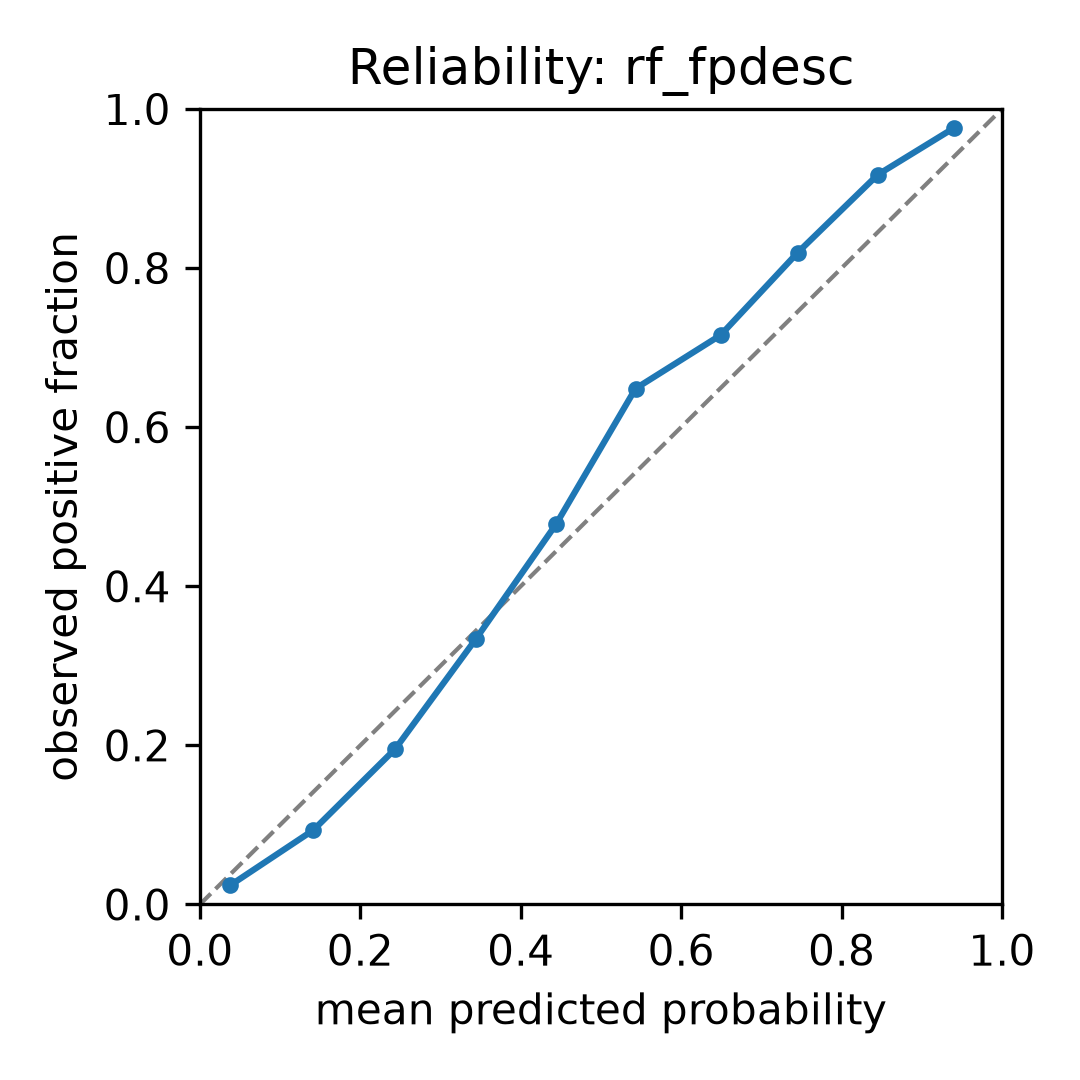
\includegraphics[width=0.46\textwidth]{calibration_rf_fpdesc.png}\hfill
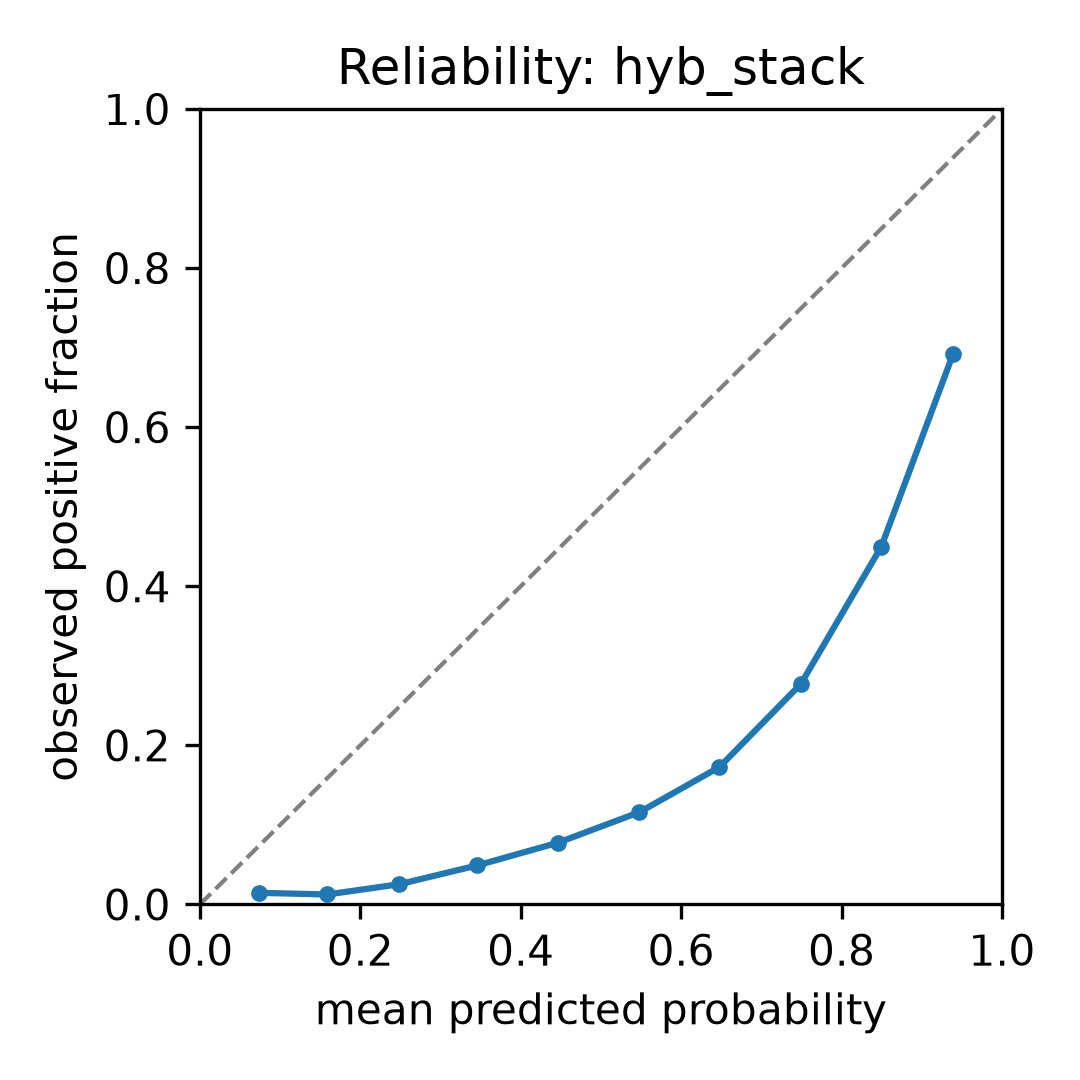
\includegraphics[width=0.46\textwidth]{calibration_hyb_stack.png}
\caption{Reliability diagrams: \code{rf\_fpdesc} (left) tracks the diagonal closely;
\code{hyb\_stack} (right) lies far below it, over-predicting toxicity at every probability level
despite ranking just as well.}
\label{fig:calibration}
\end{figure*}

\subsection{Scope of the validation}
The scorer excludes missing labels, but the data still carries assay noise and non-random
missingness. Scaffold splitting is a more demanding generalization test than a random split, but
it is neither prospective nor external validation. The statistical comparisons rest on 12
endpoints and are exploratory. Conclusions should be confirmed on additional data before any
deployment.

%--------------------------------------------------------------------
\section{Interpretability}
\label{sec:interpretability}
%--------------------------------------------------------------------
\subsection{Method}
For SR-MMP (mitochondrial membrane potential), the endpoint with the most positives, we take the
frozen \code{mpnn} run on \code{scaffold\_det} seed 0 and attribute its predictions to atoms with
GNNExplainer~\citep{ying2019gnnexplainer}, which learns a mask over the nodes of one molecule that
preserves the model's logit for that one endpoint. The molecules are not chosen by hand: they are
the five most confident true positives and the five most confident false positives on the
\emph{test} part, read from the committed prediction file, so the structures below are the ones
the reported numbers were computed from. Weights are rendered over the structure with
\code{rdkit.Chem.Draw.SimilarityMaps} (Fig.~\ref{fig:interp}); green marks atoms the logit leans
on.

\subsection{What the model keys on when it is right}
Three chemotypes dominate the confident true positives. Two are fused planar polyaromatics, where
the attribution spreads evenly over the ring system rather than concentrating on a substituent:
the model has learned the aromatic core itself. One is a di-iodinated salicylanilide, a structural
class whose members act as protonophoric uncouplers; for an assay that measures mitochondrial
membrane potential an uncoupler is a mechanistically appropriate positive, and the attribution
falls on the halogenated phenol ring rather than on the amide linker. The remaining two are a
polyene amide and a hindered bisphenol. This is not proof that the model reasons mechanistically,
but the atoms it leans on are the ones a chemist would point at.

\subsection{What the model keys on when it is wrong}
The confident false positives are the more useful half, and they separate into two groups that
each explain a failure mode rather than a one-off mistake.

\begin{itemize}
  \item \textbf{Polyphenols.} Two of the five are polyhydroxylated: a galloyl ester of a
        flavan-3-ol and a fused dihydroxy-lactone polyphenol. The attribution concentrates on the
        galloyl and catechol groups. Compounds of this class are habitual actives across
        unrelated screens --- they are redox-active and aggregation-prone, the profile of an
        assay-interference compound. The model has learned a chemotype that genuinely correlates
        with being \emph{called} active in screening data, and applies it to molecules this
        particular assay scored negative.
  \item \textbf{Lipophilic fused-ring scaffolds.} Two others are a sterol and a triterpenoid
        ester, and the third is an unsubstituted fused polyaromatic. These share ring topology
        with the true positives above while lacking the substituents that drive the real actives,
        so a model keyed on ``large fused ring system'' fires on them. This is the scaffold-split
        failure mode made visible: the test set holds ring systems the training set never showed,
        and the model generalises its polyaromatic rule too far.
\end{itemize}

Both groups say the same thing from different directions. The strongest feature the graph model
has extracted for SR-MMP is a coarse one --- extended fused ring systems and electron-rich
phenols --- informative enough to rank well and blunt enough to misfire on unseen chemistry. That
is consistent with the calibration result of Section~\ref{sec:validation}: the model orders
molecules better than it estimates their probabilities.

\begin{figure}[t]
\centering
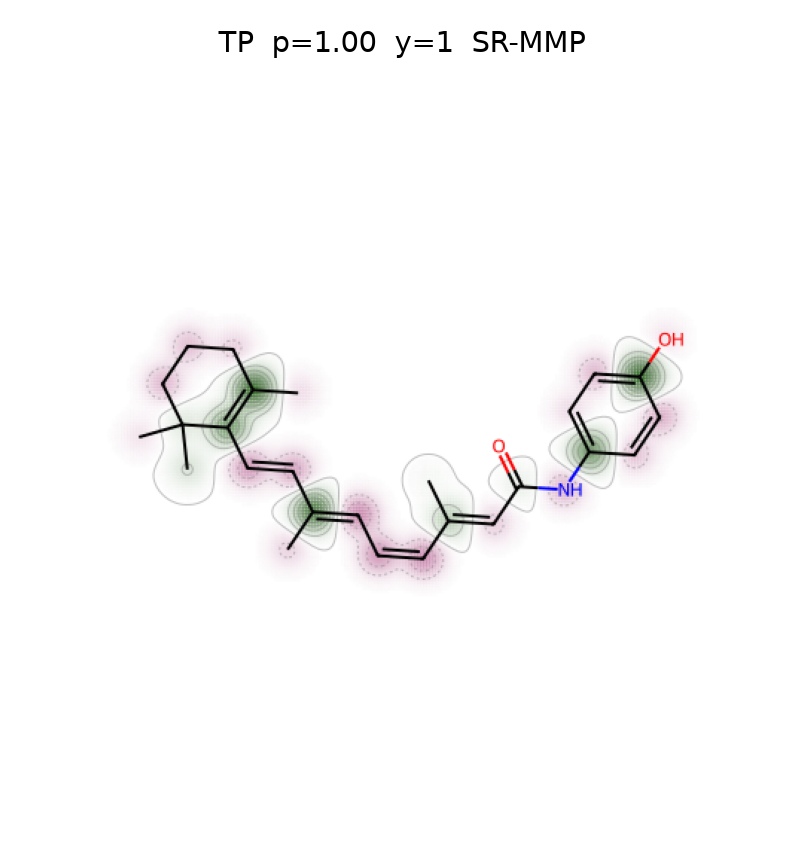
\includegraphics[width=0.47\columnwidth]{interpret_mpnn_SR-MMP_tp1.png}\hfill
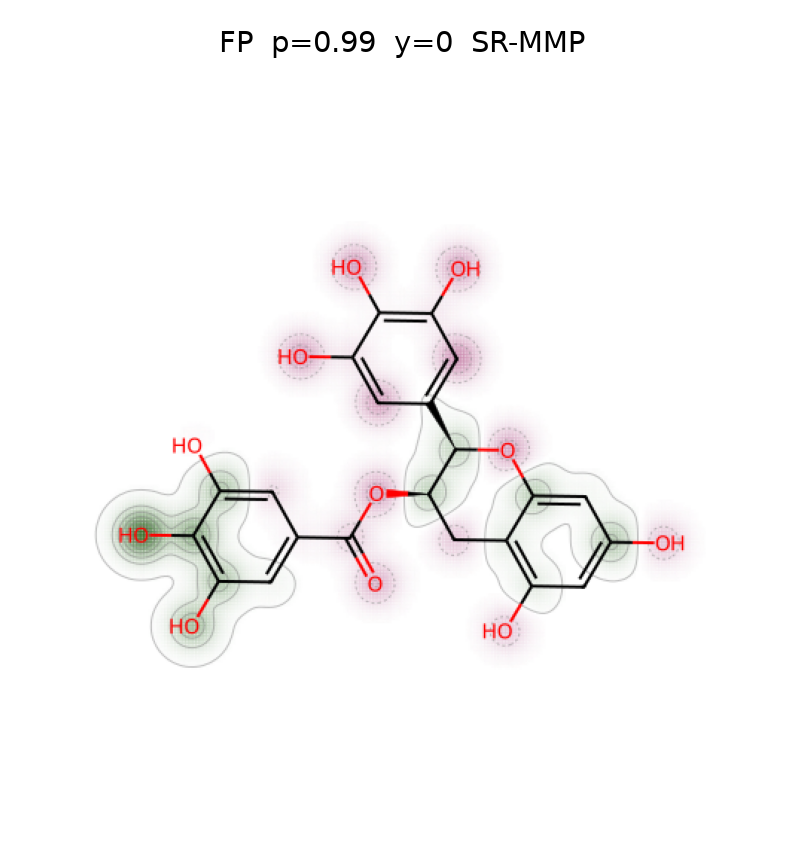
\includegraphics[width=0.47\columnwidth]{interpret_mpnn_SR-MMP_fp2.png}
\caption{Atom attributions on SR-MMP (\code{mpnn}, \code{scaffold\_det}, seed 0). Left: a
confident true positive. Right: a confident false positive, a galloyl polyphenol, where the
weight falls on the galloyl group. Green marks atoms the endpoint's logit relies on.}
\label{fig:interp}
\end{figure}

\subsection{What a saliency map does not prove}
A weight means the model's score for \emph{this} molecule drops when that atom is masked. It is
evidence about one model on one input, not a causal claim about toxicity, and not a claim that the
highlighted substructure is a toxicophore. Different explainers optimise different objectives and
can disagree on the same prediction, and GNNExplainer returns a soft mask whose magnitude is not
comparable across molecules without the centring we apply. We therefore use the maps as a
debugging instrument --- they are how the two failure groups above were found --- and not as a
result in their own right. The fingerprint side of the same question is handled by the XGBoost
gain analysis of Phase 1, which attributes to Morgan bits rather than atoms; the two views agree
that polyaromatic and phenolic environments carry most of the signal for this endpoint.

%--------------------------------------------------------------------
\section{Discussion}
%--------------------------------------------------------------------
Returning to the two questions of the introduction.

\textbf{Q1: do graph models improve on engineered features?} Partly. They beat every
fingerprint-only model on every split family, so the graph formalism recovers signal that a
fixed substructure vocabulary misses. They do not beat the fingerprint-plus-descriptor random
forest, on any split family, by any of ROC-AUC, PR-AUC or calibration. This reproduces
\citet{yang2019analyzing}'s warning on our data. Two caveats cut in the models' favour: the
tuning budget was 12 configurations per architecture on a single seed, and the MPNN ablations
show that several one-factor changes to the selected configuration improve it --- the frozen
configuration is demonstrably not the best MPNN in reach. A fair summary is that graph networks
are competitive with, not superior to, well-engineered features at this data scale and this
tuning budget.

\textbf{Q2: does combining representations help, and does coupling matter?} Yes, and
decisively. The three hybrids differ \emph{only} in how tightly the parents are coupled, and
they order inversely to that coupling: loose probability stacking is best (0.836), frozen
embeddings next (0.830), end-to-end fusion worst (0.802). Tight coupling exposes the combined
model to the weaker parent's failure modes --- here, a 256-unit encoder fine-tuned at
$10^{-3}$ that degrades within a few epochs --- while loose coupling lets each parent contribute
only what it is good at. The practical lesson for a project at this scale is that the cheapest
combination is also the most effective one.

The data also disciplines the stated rationale. We predicted that hybrids would help most on
sparse endpoints and novel scaffolds; measured, the stacking gain is real against its parents
but does not beat \code{rf\_fpdesc} in either regime. What stacking buys is error-profile
averaging, which is a weaker and more general claim than the one we set out to test --- and it
is the claim the evidence supports.

%--------------------------------------------------------------------
\section{Limitations}
%--------------------------------------------------------------------
The Phase~1 limitations carry over unchanged: Tox21 assays are in-vitro screens, not organism
toxicity; labels are noisy (44 conflicting duplicate pairs) and heavily missing (17\% of the
matrix, not at random); several endpoints have very few positives; and a scaffold split, while
much harder than a random split, is still not prospective validation. The Phase~2 additions
carry their own:

\begin{itemize}
\item \textbf{One tuning seed.} Hyper-parameters were chosen with seed 0 on \code{scaffold\_det}
validation only. Differences between neighbouring configurations smaller than the seed-to-seed
spread in the tables should not be over-interpreted, and the ablations suggest the selected MPNN
configuration is sub-optimal.
\item \textbf{Ablations are MPNN-based.} The fusion graph branch and the embedding features use
the tuned MPNN only; conclusions about combining branches may not transfer to GCN or
AttentiveFP encoders.
\item \textbf{Hybrid parents share their history.} The fusion and embedding hybrids warm-start
from the MPNN checkpoint of the same split and seed, which was itself early-stopped on that
split's validation set. This is the same information the GNN parent had, so the comparison
against the parent is fair, but every model in this comparison has seen validation through early
stopping or model selection.
\item \textbf{Statistics are exploratory.} The Wilcoxon tests run over 12 endpoints and many
model pairs without multiplicity correction.
\item \textbf{Calibration is reported, not fixed.} No post-hoc calibration was applied, so the
probability outputs of the deep and stacked models are not deployment-ready.
\item \textbf{Compute budget.} All training is single-machine CPU; the GNN hyper-parameter grid
(36 configurations) and the hybrid runs are small by deep-learning standards.
\end{itemize}

%--------------------------------------------------------------------
\section{Conclusion}
%--------------------------------------------------------------------
This phase compared fingerprint-based classical models with GCN, MPNN and AttentiveFP, and with
three hybrid combinations of the two families, on 12 Tox21 endpoints under one shared data
pipeline, seven shared splits and a single masked scorer.

The graph models perform competitively on scaffold splits and beat every fingerprint-only
baseline, but the fingerprint-plus-descriptor random forest remains the strongest single model
on every split family and is also the best calibrated by a wide margin. Probability stacking was
the most successful hybrid: it improved on both of its parents and was the only model the
exploratory paired test could not separate from that baseline, though it is the worst-calibrated
model in the comparison. End-to-end fusion gave no benefit under the tested training recipe, and
its ablations identify the fine-tuned encoder as the cause.

The supported conclusion is measured rather than promotional: graph-learned representations are
useful complements to engineered chemical features, not automatic replacements for them, and the
value of combining representations depends on how loosely they are coupled. The most productive
next steps are a wider multi-seed tuning budget for the graph models, post-hoc calibration of
the stacked model, a lower learning rate with a frozen warm-up for end-to-end fusion, and
evaluation on external or prospective data.

%--------------------------------------------------------------------
\bibliographystyle{plainnat}
\bibliography{references_gnn,../phase1/references}

\appendix
\clearpage
%--------------------------------------------------------------------
\section{Full sparse-versus-dense endpoint results}
\label{app:sparse}
%--------------------------------------------------------------------
\begin{table}[h]
\centering
\caption{Test ROC-AUC and PR-AUC on the 4 sparsest versus the 4 densest endpoints
(\code{scaffold\_det}, mean $\pm$ std over seeds), all twelve models.}
\small
\begin{tabular}{llcc}
\toprule
model & endpoints & ROC-AUC & PR-AUC \\
\midrule
afp & 4 sparsest & 0.764 $\pm$ 0.040 & 0.342 $\pm$ 0.077 \\
afp & 4 densest & 0.778 $\pm$ 0.085 & 0.477 $\pm$ 0.106 \\
gcn & 4 sparsest & 0.740 $\pm$ 0.051 & 0.330 $\pm$ 0.073 \\
gcn & 4 densest & 0.760 $\pm$ 0.081 & 0.474 $\pm$ 0.093 \\
mpnn & 4 sparsest & 0.728 $\pm$ 0.040 & 0.270 $\pm$ 0.077 \\
mpnn & 4 densest & 0.745 $\pm$ 0.070 & 0.426 $\pm$ 0.094 \\
hyb\_embxgb & 4 sparsest & 0.742 $\pm$ 0.043 & 0.295 $\pm$ 0.085 \\
hyb\_embxgb & 4 densest & 0.757 $\pm$ 0.073 & 0.464 $\pm$ 0.087 \\
hyb\_fusion & 4 sparsest & 0.760 $\pm$ 0.034 & 0.284 $\pm$ 0.099 \\
hyb\_fusion & 4 densest & 0.751 $\pm$ 0.063 & 0.430 $\pm$ 0.085 \\
hyb\_stack & 4 sparsest & 0.755 $\pm$ 0.022 & 0.369 $\pm$ 0.059 \\
hyb\_stack & 4 densest & 0.789 $\pm$ 0.081 & 0.536 $\pm$ 0.090 \\
lr\_fp & 4 sparsest & 0.709 $\pm$ 0.022 & 0.335 $\pm$ 0.062 \\
lr\_fp & 4 densest & 0.733 $\pm$ 0.069 & 0.419 $\pm$ 0.097 \\
lr\_fpdesc & 4 sparsest & 0.717 $\pm$ 0.046 & 0.255 $\pm$ 0.075 \\
lr\_fpdesc & 4 densest & 0.735 $\pm$ 0.093 & 0.429 $\pm$ 0.124 \\
rf\_fp & 4 sparsest & 0.765 $\pm$ 0.029 & 0.386 $\pm$ 0.042 \\
rf\_fp & 4 densest & 0.744 $\pm$ 0.052 & 0.469 $\pm$ 0.086 \\
rf\_fpdesc & 4 sparsest & 0.786 $\pm$ 0.046 & 0.385 $\pm$ 0.072 \\
rf\_fpdesc & 4 densest & 0.791 $\pm$ 0.073 & 0.532 $\pm$ 0.084 \\
xgb\_fp & 4 sparsest & 0.708 $\pm$ 0.033 & 0.329 $\pm$ 0.037 \\
xgb\_fp & 4 densest & 0.712 $\pm$ 0.057 & 0.404 $\pm$ 0.061 \\
xgb\_fpdesc & 4 sparsest & 0.754 $\pm$ 0.078 & 0.373 $\pm$ 0.087 \\
xgb\_fpdesc & 4 densest & 0.783 $\pm$ 0.082 & 0.528 $\pm$ 0.093 \\
\bottomrule
\end{tabular}
\end{table}

\clearpage
%--------------------------------------------------------------------
\section{Full similarity-bin results}
\label{app:simbins}
%--------------------------------------------------------------------
\begin{table}[h]
\centering
\caption{Test ROC-AUC (all 12 tasks pooled, missing labels masked) by maximum Tanimoto
similarity of each test molecule to the training set (\code{scaffold\_det}, mean $\pm$ std over
seeds). Bin sizes: 172, 365 and 235 molecules.}
\small
\begin{tabular}{lccc}
\toprule
model & $[0,\,0.3)$ & $[0.3,\,0.5)$ & $[0.5,\,1]$ \\
\midrule
afp & 0.703 $\pm$ 0.007 & 0.798 $\pm$ 0.008 & 0.846 $\pm$ 0.007 \\
gcn & 0.703 $\pm$ 0.009 & 0.787 $\pm$ 0.007 & 0.846 $\pm$ 0.005 \\
mpnn & 0.645 $\pm$ 0.007 & 0.769 $\pm$ 0.015 & 0.828 $\pm$ 0.014 \\
hyb\_embxgb & 0.660 $\pm$ 0.036 & 0.770 $\pm$ 0.006 & 0.835 $\pm$ 0.009 \\
hyb\_fusion & 0.657 $\pm$ 0.032 & 0.766 $\pm$ 0.021 & 0.812 $\pm$ 0.033 \\
hyb\_stack & 0.724 $\pm$ 0.019 & 0.787 $\pm$ 0.007 & 0.840 $\pm$ 0.006 \\
lr\_fp & 0.662 $\pm$ 0.000 & 0.723 $\pm$ 0.000 & 0.819 $\pm$ 0.000 \\
lr\_fpdesc & 0.704 $\pm$ 0.000 & 0.740 $\pm$ 0.000 & 0.816 $\pm$ 0.000 \\
rf\_fp & 0.654 $\pm$ 0.013 & 0.723 $\pm$ 0.006 & 0.823 $\pm$ 0.001 \\
rf\_fpdesc & \textbf{0.751 $\pm$ 0.009} & \textbf{0.810 $\pm$ 0.005} & \textbf{0.865 $\pm$ 0.002} \\
xgb\_fp & 0.639 $\pm$ 0.017 & 0.694 $\pm$ 0.026 & 0.797 $\pm$ 0.013 \\
xgb\_fpdesc & 0.749 $\pm$ 0.014 & 0.773 $\pm$ 0.022 & 0.829 $\pm$ 0.013 \\
\bottomrule
\end{tabular}
\end{table}

\clearpage
%--------------------------------------------------------------------
\onecolumn
\section{Full Wilcoxon signed-rank matrix}
\label{app:wilcoxon}
%--------------------------------------------------------------------
All pairs on the balanced scaffold family (\code{scaffold\_s0}--\code{scaffold\_s2}; 12 paired
endpoint means, each averaged over its 3 runs). $^{*}$/$^{**}$: $p<0.05$ / $p<0.01$.
Exploratory: many pairs, no multiplicity correction.

\begin{longtable}{llccl}
\toprule
model $a$ & model $b$ & ROC-AUC $a$ & ROC-AUC $b$ & $p$ \\
\midrule
\endfirsthead
\toprule
model $a$ & model $b$ & ROC-AUC $a$ & ROC-AUC $b$ & $p$ \\
\midrule
\endhead
\bottomrule
\endfoot
afp & hyb\_embxgb & 0.828 & 0.830 & 0.733 \\
afp & hyb\_fusion & 0.828 & 0.802 & 0.005$^{**}$ \\
afp & hyb\_stack & 0.828 & 0.836 & 0.077 \\
afp & mpnn & 0.828 & 0.813 & 0.016$^{*}$ \\
afp & rf\_fpdesc & 0.828 & 0.839 & 0.034$^{*}$ \\
afp & xgb\_fpdesc & 0.828 & 0.813 & 0.110 \\
gcn & hyb\_embxgb & 0.826 & 0.830 & 0.380 \\
gcn & hyb\_fusion & 0.826 & 0.802 & 0.007$^{**}$ \\
gcn & hyb\_stack & 0.826 & 0.836 & 0.052 \\
gcn & mpnn & 0.826 & 0.813 & 0.064 \\
gcn & rf\_fpdesc & 0.826 & 0.839 & 0.021$^{*}$ \\
gcn & xgb\_fpdesc & 0.826 & 0.813 & 0.233 \\
hyb\_embxgb & hyb\_fusion & 0.830 & 0.802 & 0.000$^{**}$ \\
hyb\_embxgb & hyb\_stack & 0.830 & 0.836 & 0.129 \\
hyb\_embxgb & lr\_fp & 0.830 & 0.775 & 0.000$^{**}$ \\
hyb\_embxgb & lr\_fpdesc & 0.830 & 0.788 & 0.002$^{**}$ \\
hyb\_embxgb & mpnn & 0.830 & 0.813 & 0.005$^{**}$ \\
hyb\_embxgb & rf\_fp & 0.830 & 0.803 & 0.005$^{**}$ \\
hyb\_embxgb & rf\_fpdesc & 0.830 & 0.839 & 0.151 \\
hyb\_embxgb & xgb\_fp & 0.830 & 0.767 & 0.000$^{**}$ \\
hyb\_embxgb & xgb\_fpdesc & 0.830 & 0.813 & 0.077 \\
hyb\_fusion & hyb\_stack & 0.802 & 0.836 & 0.001$^{**}$ \\
hyb\_fusion & lr\_fp & 0.802 & 0.775 & 0.005$^{**}$ \\
hyb\_fusion & lr\_fpdesc & 0.802 & 0.788 & 0.129 \\
hyb\_fusion & mpnn & 0.802 & 0.813 & 0.077 \\
hyb\_fusion & rf\_fp & 0.802 & 0.803 & 0.910 \\
hyb\_fusion & rf\_fpdesc & 0.802 & 0.839 & 0.001$^{**}$ \\
hyb\_fusion & xgb\_fp & 0.802 & 0.767 & 0.002$^{**}$ \\
hyb\_fusion & xgb\_fpdesc & 0.802 & 0.813 & 0.266 \\
hyb\_stack & lr\_fp & 0.836 & 0.775 & 0.000$^{**}$ \\
hyb\_stack & lr\_fpdesc & 0.836 & 0.788 & 0.001$^{**}$ \\
hyb\_stack & mpnn & 0.836 & 0.813 & 0.000$^{**}$ \\
hyb\_stack & rf\_fp & 0.836 & 0.803 & 0.000$^{**}$ \\
hyb\_stack & rf\_fpdesc & 0.836 & 0.839 & 0.470 \\
hyb\_stack & xgb\_fp & 0.836 & 0.767 & 0.000$^{**}$ \\
hyb\_stack & xgb\_fpdesc & 0.836 & 0.813 & 0.005$^{**}$ \\
lr\_fp & mpnn & 0.775 & 0.813 & 0.001$^{**}$ \\
lr\_fp & rf\_fpdesc & 0.775 & 0.839 & 0.000$^{**}$ \\
lr\_fp & xgb\_fpdesc & 0.775 & 0.813 & 0.001$^{**}$ \\
lr\_fpdesc & mpnn & 0.788 & 0.813 & 0.052 \\
lr\_fpdesc & rf\_fpdesc & 0.788 & 0.839 & 0.001$^{**}$ \\
lr\_fpdesc & xgb\_fpdesc & 0.788 & 0.813 & 0.009$^{**}$ \\
mpnn & rf\_fp & 0.813 & 0.803 & 0.233 \\
mpnn & rf\_fpdesc & 0.813 & 0.839 & 0.002$^{**}$ \\
mpnn & xgb\_fp & 0.813 & 0.767 & 0.000$^{**}$ \\
mpnn & xgb\_fpdesc & 0.813 & 0.813 & 0.850 \\
rf\_fp & rf\_fpdesc & 0.803 & 0.839 & 0.001$^{**}$ \\
rf\_fp & xgb\_fpdesc & 0.803 & 0.813 & 0.339 \\
rf\_fpdesc & xgb\_fp & 0.839 & 0.767 & 0.000$^{**}$ \\
rf\_fpdesc & xgb\_fpdesc & 0.839 & 0.813 & 0.002$^{**}$ \\
xgb\_fp & xgb\_fpdesc & 0.767 & 0.813 & 0.002$^{**}$ \\
\end{longtable}
\twocolumn

\clearpage
%--------------------------------------------------------------------
\section{Reproducibility}
\label{app:repro}
%--------------------------------------------------------------------
Every number in this report is read from a committed results file; nothing was measured outside
\code{tox.metrics}. The pipeline is reproduced in three stages from a clean checkout:

\begin{enumerate}
\item \code{./run\_all.sh} --- download and clean the data, build the seven splits, compute
fingerprints and descriptors, train and score the classical grid.
\item \code{./run\_gnn.sh} --- tune GCN/MPNN/AttentiveFP on \code{scaffold\_det} validation
(36 configurations), train the frozen-configuration grid (3 models $\times$ 3 split families
$\times$ 3 seeds $=$ 27 runs) and score it, then run the 27 MPNN ablation runs.
\item \code{bash run\_hybrid.sh} --- the three hybrid variants on the same 9 (split, seed)
pairs, the hybrid ablations, the sparse/dense and similarity-bin analyses, and the technical
validation (Wilcoxon tests, calibration).
\end{enumerate}

All three stages are resumable: a run whose prediction file already exists is skipped. Results
are written under \code{results/} as per-run metrics (\code{results/metrics/}), aggregated
summaries (\code{results/summary.csv}, \code{results/headline.csv}) and validation outputs
(\code{results/validation/}). The tables in this report are regenerated with
\code{python -m tox.gnn\_report} and \code{python -m tox.hybrid\_report}.

\end{document}
